% Options for packages loaded elsewhere
\PassOptionsToPackage{unicode}{hyperref}
\PassOptionsToPackage{hyphens}{url}
%
\documentclass[
  man,floatsintext]{apa6}
\usepackage{amsmath,amssymb}
\usepackage{iftex}
\ifPDFTeX
  \usepackage[T1]{fontenc}
  \usepackage[utf8]{inputenc}
  \usepackage{textcomp} % provide euro and other symbols
\else % if luatex or xetex
  \usepackage{unicode-math} % this also loads fontspec
  \defaultfontfeatures{Scale=MatchLowercase}
  \defaultfontfeatures[\rmfamily]{Ligatures=TeX,Scale=1}
\fi
\usepackage{lmodern}
\ifPDFTeX\else
  % xetex/luatex font selection
\fi
% Use upquote if available, for straight quotes in verbatim environments
\IfFileExists{upquote.sty}{\usepackage{upquote}}{}
\IfFileExists{microtype.sty}{% use microtype if available
  \usepackage[]{microtype}
  \UseMicrotypeSet[protrusion]{basicmath} % disable protrusion for tt fonts
}{}
\makeatletter
\@ifundefined{KOMAClassName}{% if non-KOMA class
  \IfFileExists{parskip.sty}{%
    \usepackage{parskip}
  }{% else
    \setlength{\parindent}{0pt}
    \setlength{\parskip}{6pt plus 2pt minus 1pt}}
}{% if KOMA class
  \KOMAoptions{parskip=half}}
\makeatother
\usepackage{xcolor}
\usepackage{color}
\usepackage{fancyvrb}
\newcommand{\VerbBar}{|}
\newcommand{\VERB}{\Verb[commandchars=\\\{\}]}
\DefineVerbatimEnvironment{Highlighting}{Verbatim}{commandchars=\\\{\}}
% Add ',fontsize=\small' for more characters per line
\usepackage{framed}
\definecolor{shadecolor}{RGB}{248,248,248}
\newenvironment{Shaded}{\begin{snugshade}}{\end{snugshade}}
\newcommand{\AlertTok}[1]{\textcolor[rgb]{0.94,0.16,0.16}{#1}}
\newcommand{\AnnotationTok}[1]{\textcolor[rgb]{0.56,0.35,0.01}{\textbf{\textit{#1}}}}
\newcommand{\AttributeTok}[1]{\textcolor[rgb]{0.13,0.29,0.53}{#1}}
\newcommand{\BaseNTok}[1]{\textcolor[rgb]{0.00,0.00,0.81}{#1}}
\newcommand{\BuiltInTok}[1]{#1}
\newcommand{\CharTok}[1]{\textcolor[rgb]{0.31,0.60,0.02}{#1}}
\newcommand{\CommentTok}[1]{\textcolor[rgb]{0.56,0.35,0.01}{\textit{#1}}}
\newcommand{\CommentVarTok}[1]{\textcolor[rgb]{0.56,0.35,0.01}{\textbf{\textit{#1}}}}
\newcommand{\ConstantTok}[1]{\textcolor[rgb]{0.56,0.35,0.01}{#1}}
\newcommand{\ControlFlowTok}[1]{\textcolor[rgb]{0.13,0.29,0.53}{\textbf{#1}}}
\newcommand{\DataTypeTok}[1]{\textcolor[rgb]{0.13,0.29,0.53}{#1}}
\newcommand{\DecValTok}[1]{\textcolor[rgb]{0.00,0.00,0.81}{#1}}
\newcommand{\DocumentationTok}[1]{\textcolor[rgb]{0.56,0.35,0.01}{\textbf{\textit{#1}}}}
\newcommand{\ErrorTok}[1]{\textcolor[rgb]{0.64,0.00,0.00}{\textbf{#1}}}
\newcommand{\ExtensionTok}[1]{#1}
\newcommand{\FloatTok}[1]{\textcolor[rgb]{0.00,0.00,0.81}{#1}}
\newcommand{\FunctionTok}[1]{\textcolor[rgb]{0.13,0.29,0.53}{\textbf{#1}}}
\newcommand{\ImportTok}[1]{#1}
\newcommand{\InformationTok}[1]{\textcolor[rgb]{0.56,0.35,0.01}{\textbf{\textit{#1}}}}
\newcommand{\KeywordTok}[1]{\textcolor[rgb]{0.13,0.29,0.53}{\textbf{#1}}}
\newcommand{\NormalTok}[1]{#1}
\newcommand{\OperatorTok}[1]{\textcolor[rgb]{0.81,0.36,0.00}{\textbf{#1}}}
\newcommand{\OtherTok}[1]{\textcolor[rgb]{0.56,0.35,0.01}{#1}}
\newcommand{\PreprocessorTok}[1]{\textcolor[rgb]{0.56,0.35,0.01}{\textit{#1}}}
\newcommand{\RegionMarkerTok}[1]{#1}
\newcommand{\SpecialCharTok}[1]{\textcolor[rgb]{0.81,0.36,0.00}{\textbf{#1}}}
\newcommand{\SpecialStringTok}[1]{\textcolor[rgb]{0.31,0.60,0.02}{#1}}
\newcommand{\StringTok}[1]{\textcolor[rgb]{0.31,0.60,0.02}{#1}}
\newcommand{\VariableTok}[1]{\textcolor[rgb]{0.00,0.00,0.00}{#1}}
\newcommand{\VerbatimStringTok}[1]{\textcolor[rgb]{0.31,0.60,0.02}{#1}}
\newcommand{\WarningTok}[1]{\textcolor[rgb]{0.56,0.35,0.01}{\textbf{\textit{#1}}}}
\usepackage{graphicx}
\makeatletter
\def\maxwidth{\ifdim\Gin@nat@width>\linewidth\linewidth\else\Gin@nat@width\fi}
\def\maxheight{\ifdim\Gin@nat@height>\textheight\textheight\else\Gin@nat@height\fi}
\makeatother
% Scale images if necessary, so that they will not overflow the page
% margins by default, and it is still possible to overwrite the defaults
% using explicit options in \includegraphics[width, height, ...]{}
\setkeys{Gin}{width=\maxwidth,height=\maxheight,keepaspectratio}
% Set default figure placement to htbp
\makeatletter
\def\fps@figure{htbp}
\makeatother
\setlength{\emergencystretch}{3em} % prevent overfull lines
\providecommand{\tightlist}{%
  \setlength{\itemsep}{0pt}\setlength{\parskip}{0pt}}
\setcounter{secnumdepth}{-\maxdimen} % remove section numbering
% Make \paragraph and \subparagraph free-standing
\ifx\paragraph\undefined\else
  \let\oldparagraph\paragraph
  \renewcommand{\paragraph}[1]{\oldparagraph{#1}\mbox{}}
\fi
\ifx\subparagraph\undefined\else
  \let\oldsubparagraph\subparagraph
  \renewcommand{\subparagraph}[1]{\oldsubparagraph{#1}\mbox{}}
\fi
% definitions for citeproc citations
\NewDocumentCommand\citeproctext{}{}
\NewDocumentCommand\citeproc{mm}{%
  \begingroup\def\citeproctext{#2}\cite{#1}\endgroup}
\makeatletter
 % allow citations to break across lines
 \let\@cite@ofmt\@firstofone
 % avoid brackets around text for \cite:
 \def\@biblabel#1{}
 \def\@cite#1#2{{#1\if@tempswa , #2\fi}}
\makeatother
\newlength{\cslhangindent}
\setlength{\cslhangindent}{1.5em}
\newlength{\csllabelwidth}
\setlength{\csllabelwidth}{3em}
\newenvironment{CSLReferences}[2] % #1 hanging-indent, #2 entry-spacing
 {\begin{list}{}{%
  \setlength{\itemindent}{0pt}
  \setlength{\leftmargin}{0pt}
  \setlength{\parsep}{0pt}
  % turn on hanging indent if param 1 is 1
  \ifodd #1
   \setlength{\leftmargin}{\cslhangindent}
   \setlength{\itemindent}{-1\cslhangindent}
  \fi
  % set entry spacing
  \setlength{\itemsep}{#2\baselineskip}}}
 {\end{list}}
\usepackage{calc}
\newcommand{\CSLBlock}[1]{\hfill\break#1\hfill\break}
\newcommand{\CSLLeftMargin}[1]{\parbox[t]{\csllabelwidth}{\strut#1\strut}}
\newcommand{\CSLRightInline}[1]{\parbox[t]{\linewidth - \csllabelwidth}{\strut#1\strut}}
\newcommand{\CSLIndent}[1]{\hspace{\cslhangindent}#1}
\ifLuaTeX
\usepackage[bidi=basic]{babel}
\else
\usepackage[bidi=default]{babel}
\fi
\babelprovide[main,import]{english}
% get rid of language-specific shorthands (see #6817):
\let\LanguageShortHands\languageshorthands
\def\languageshorthands#1{}
% Manuscript styling
\usepackage{upgreek}
\captionsetup{font=singlespacing,justification=justified}

% Table formatting
\usepackage{longtable}
\usepackage{lscape}
% \usepackage[counterclockwise]{rotating}   % Landscape page setup for large tables
\usepackage{multirow}		% Table styling
\usepackage{tabularx}		% Control Column width
\usepackage[flushleft]{threeparttable}	% Allows for three part tables with a specified notes section
\usepackage{threeparttablex}            % Lets threeparttable work with longtable

% Create new environments so endfloat can handle them
% \newenvironment{ltable}
%   {\begin{landscape}\centering\begin{threeparttable}}
%   {\end{threeparttable}\end{landscape}}
\newenvironment{lltable}{\begin{landscape}\centering\begin{ThreePartTable}}{\end{ThreePartTable}\end{landscape}}

% Enables adjusting longtable caption width to table width
% Solution found at http://golatex.de/longtable-mit-caption-so-breit-wie-die-tabelle-t15767.html
\makeatletter
\newcommand\LastLTentrywidth{1em}
\newlength\longtablewidth
\setlength{\longtablewidth}{1in}
\newcommand{\getlongtablewidth}{\begingroup \ifcsname LT@\roman{LT@tables}\endcsname \global\longtablewidth=0pt \renewcommand{\LT@entry}[2]{\global\advance\longtablewidth by ##2\relax\gdef\LastLTentrywidth{##2}}\@nameuse{LT@\roman{LT@tables}} \fi \endgroup}

% \setlength{\parindent}{0.5in}
% \setlength{\parskip}{0pt plus 0pt minus 0pt}

% Overwrite redefinition of paragraph and subparagraph by the default LaTeX template
% See https://github.com/crsh/papaja/issues/292
\makeatletter
\renewcommand{\paragraph}{\@startsection{paragraph}{4}{\parindent}%
  {0\baselineskip \@plus 0.2ex \@minus 0.2ex}%
  {-1em}%
  {\normalfont\normalsize\bfseries\itshape\typesectitle}}

\renewcommand{\subparagraph}[1]{\@startsection{subparagraph}{5}{1em}%
  {0\baselineskip \@plus 0.2ex \@minus 0.2ex}%
  {-\z@\relax}%
  {\normalfont\normalsize\itshape\hspace{\parindent}{#1}\textit{\addperi}}{\relax}}
\makeatother

% \usepackage{etoolbox}
\makeatletter
\patchcmd{\HyOrg@maketitle}
  {\section{\normalfont\normalsize\abstractname}}
  {\section*{\normalfont\normalsize\abstractname}}
  {}{\typeout{Failed to patch abstract.}}
\patchcmd{\HyOrg@maketitle}
  {\section{\protect\normalfont{\@title}}}
  {\section*{\protect\normalfont{\@title}}}
  {}{\typeout{Failed to patch title.}}
\makeatother

\usepackage{xpatch}
\makeatletter
\xapptocmd\appendix
  {\xapptocmd\section
    {\addcontentsline{toc}{section}{\appendixname\ifoneappendix\else~\theappendix\fi\\: #1}}
    {}{\InnerPatchFailed}%
  }
{}{\PatchFailed}
\keywords{ordinal, simulations, power\newline\indent Word count: X}
\usepackage{csquotes}
\ifLuaTeX
  \usepackage{selnolig}  % disable illegal ligatures
\fi
\IfFileExists{bookmark.sty}{\usepackage{bookmark}}{\usepackage{hyperref}}
\IfFileExists{xurl.sty}{\usepackage{xurl}}{} % add URL line breaks if available
\urlstyle{same}
\hypersetup{
  pdftitle={Ordinal regression models made easy. A tutorial on parameter interpretation, data simulation, and power analysis.},
  pdfauthor={Filippo Gambarota1 \& Gianmarco Altoè1},
  pdflang={en-EN},
  pdfkeywords={ordinal, simulations, power},
  hidelinks,
  pdfcreator={LaTeX via pandoc}}

\title{Ordinal regression models made easy. A tutorial on parameter interpretation, data simulation, and power analysis.}
\author{Filippo Gambarota\textsuperscript{1} \& Gianmarco Altoè\textsuperscript{1}}
\date{}


\shorttitle{Ordinal regression models made easy}

\authornote{

The authors made the following contributions. Filippo Gambarota: Conceptualization, Writing - Original Draft Preparation, Writing - Review \& Editing, Methodology, Software; Gianmarco Altoè: Conceptualization, Writing - Review \& Editing, Supervision.

Correspondence concerning this article should be addressed to Filippo Gambarota, Via Venezia 8, 35131, Padova (Italy). E-mail: \href{mailto:filippo.gambarota@unipd.it}{\nolinkurl{filippo.gambarota@unipd.it}}

}

\affiliation{\vspace{0.5cm}\textsuperscript{1} Department of Developmental Psychology and Socialization, University of Padova, Italy}

\abstract{%
Ordinal data are very common in psychology such as Likert items, ratings or generic ordinal variables. Despite the widespread these variables are usually analyzed using metric models (e.g., standard linear regression). This approach can have important drawbacks in terms of statistical inference (e.g., reduced power) and prediction. One of the possible reason of not using ordinal regression models could be the difficulty in understanding parameters (e.g., odds ratios) or conduting a power analysis. The aim of the tutorial is presenting ordinal regression models using a simulation-based approach. In the first section we introduced the general model highlighting the crucial components and assumptions. Then we explained how to intepret the parameters for a logit and probit model. Then we proposed two way for simulating ordinal data as a function of predictors showing common research design such as a 2x2 interaction with categorical predictors and the interaction between a numeric and categorical predictor. Finally, we showed an example of power analysis using simulations that can be easily extended to complex models with multiple predictors. The tutorial is supported by a collection of custom R functions developed to simulate and understand ordinal regression models. The code to reproduce the proposed simulation, the custom R functions and other examples of ordinal regression models can be found on the online Github repository.
}



\begin{document}
\maketitle

\scriptsize

\normalsize

\scriptsize

\normalsize

\section{Introduction}\label{introduction}

Psychological research make an extensive use of ordinal data. One of the main reason is probably the usage of Likert scales (Likert, 1932). Ordinal data, as defined by Stevens (1946), belongs to a specific type of measurement scale where ordered numbers are assigned to a variable. Beyond Likert-like items, in Psychology there are several applications of ordinal scales. For instance, sociodemographic variables like educational levels or socioeconomic status, as well as general ratings such as pain severity, agreement with a statement, or the evaluation of sensory experiences (e.g., Overgaard \& Sandberg, 2021).

In contrast to nominal scales, the labels in ordinal scales are ordered. Unlike interval or ratio scales, there is no explicit assumption about the distance between labels. An example is asking people the degree of agreement about a certain statement using a scale from 1 (no agreement) to 7 (total agreement). Answering 4 compared to 2 suggest an higher agreement but we cannot affirm that there is two times the agreement compared to the second answer. Stevens (1946) and Kemp and Grace (2021) suggested that for ordinal variables is appropriate to calculate ranks-based descriptive statistics (e.g., median or percentiles) instead of metric statistics (e.g., mean or standard deviation) and using appropriate inferential tools (Agresti, 2010; e.g., N. Cliff, 1996). This distinction in terms of the appropriateness of certain descriptive statistics is also relevant when modeling data. Treating ordinal data as metric refers to assuming the labels as actual integer numbers thus assuming a fixed and know distance between levels (Liddell \& Kruschke, 2018). More generally, Norman Cliff (2016) suggests that several research questions in behavioral sciences can be considered as ordinal (\emph{is the score} \(x\) higher than the score \(y\)?) concerning variables where the most appropriate measurement scale is probably ordinal.

In Psychology especially when using item-based measures (questionnaires, surveys, etc.) the common practice is using a linear regression that makes an explicit assumption about metric features of the response variable. Liddell and Kruschke (2018) reviewed the psychological literature using Likert-based measures and reported how the majority of papers used metric-based statistical models. In the same work, Liddell and Kruschke (2018) showed examples about the potential pitfalls of metric models applied to ordinal variables (but see Robitzsch, 2020 for an alternative perspective). They reported problems in terms of lack of power, inversion of the effects (e.g., finding a negative effect when the true effect is positive) and biased estimates. While sums or averages of ordinal items could be treated as metric (Carifio \& Perla, 2008; Carifio \& Perla, 2007; but see Jamieson, 2004) Liddell and Kruschke (2018) provided some examples of potential pitfalls even in this case. In the current paper we discuss only cases where there is a single ordinal outcome (e.g., a single item, question, etc.) without considering the case of aggregating ordinal responses.

For the tutorial, we assume that the reader is familiar with basic R programming and introductory theory about linear regression. Similar to other tutorials (DeBruine \& Barr, 2021; Gambarota \& Altoè, 2023) we used few equations that are necessary to understand the model parameters and implement the Monte Carlo simulation.

In the first part we introduce the ordinal models explaining the general structure and assumptions. Then we move with model fitting and parameters interpretation. Finally we introduce the simulation approach for common research scenarios and an application to power analysis. We used R {[}Version 4.3.1; R Core Team (2023){]} for the code, figures and tables. Details about R packages an The tutorial is supported by a set of custom R functions available on Github. Other examples and model extensions along with details about used R packages are available on the Github repository (supplementary materials). For the tutorial we used the following packages.

\scriptsize

\normalsize

\subsection{Ordinal regression models}\label{ordinal-regression-models}

Despite the specific model proposed by Liddell and Kruschke (2018) proposed a specific modeling approach, there is a class of regression models that consider the ordinal nature of the response variable. The actual statistical nomenclature of \emph{ordinal regression} models can be confusing (Tutz, 2022). Tutz (2022) and Bürkner and Vuorre (2019) provide a clear and updated taxonomy of ordinal regression models.

We can identify three main types: \emph{cumulative models} (Agresti, 2010; CM, McCullagh, 1980), \emph{sequential models} (Tutz, 1990), and \emph{adjacent category models}. Among these, the cumulative model is the most widely used, assuming the existence of a latent variable categorized using a set of thresholds. The \emph{sequential model} is appropriate when modeling sequential processes. Assuming to have five response options, the sequential model assume that responding ``3'' assume a sequential process where steps ``1'' and ``2'' are already reached. A clear example is proposed by Bürkner and Vuorre (2019) where the marriage duration in years is predicted as a function of some explanatory variables. For each level of the response variable there is a latent distribution where the step between a marriage year \(k = 1\) and the next years \(k > 1\) is modeled by the sequential model. When comparing \(k\) with \(k > 1\), everything lower than \(k\) is assumed to be already reached (Tutz \& Berger, 2020).

The adjacent category model compare the category \(k\) with \(k + 1\) still assuming a latent distribution for each \(k\). As suggested by Tutz (2022) the adjacent-category model can be seen as a series of binary binomial regressions taking into account the order of the categories. Bürkner and Vuorre (2019) suggested that adjacent-category model can be chosen for its mathematical convenience and there is no a clear empirical interpretation as for the cumulative vs sequential model.

In the current paper we put the focus on the CM for several reasons. Firstly, the latent formulation of the model is particularly convenient for parameter interpretation and data simulation. The second reason is that several psychological variables can be formalized as a latent continuous variable observed as an ordinal item. Furthermore, the signal detection theory framework that is very common in experimental psychology can be implemented using a CM (e.g., DeCarlo, 2010). Figure \ref{fig:fig-explain-cumulative} depicts the overall structure of the CM.

\subsection{Model notation}\label{model-notation}

In this section we introduce some notation for the CM to be consistent with the existing literature and the \texttt{ordinal} R package (Christensen, 2022). We define \(Y_k\) as the observed ordinal variable with \(k\) levels and \(Y^\star\) is the underlying latent variable. The latent variable is segmented using \(k - 1\) thresholds \(\alpha_1, \dots, \alpha_{k - 1}\). Similarly to the generalized linear models framework (e.g., Fox, 2015), we define \(g(x) = \eta\) as the link function that maps probabilities into the linear predictor \(\eta\). To transform back \(\eta\) into probabilities we use the inverse of the link function \(x = g^{-1}(\eta)\). The specific link function define the type of model and require a different R function. For example, when assuming a Gaussian distribution (\emph{probit} link function) entails using the cumulative distribution function \(g(x) = \Phi^{-1}(x) = \eta\) and the inverse of the link function is the inverse cumulative distribution function (or quantile function) defined \(x = g^{-1}(\eta) = \Phi(\eta)\).

When modelling an ordinal variable in a cumulative link model we actually modelling the cumulative probability \(P(Y \leq k), k = 1, \dots, k - 1\)\footnote{As done by Agresti (2010), when referring to \(P(Y \leq k)\) we are implicitly conditioning on a particular \(\mathbf{X}\) value \(P(Y \leq k | \mathbf{X}_i)\)}. Equation \eqref{eq:prob-cum-model1} shows the general cumulative model including predictors \(\mathbf{X}\) and regression coefficients \(\boldsymbol{\beta}\). The minus sign in \(\mathbf{X} \boldsymbol{\beta}\) is used to interpret the \(\beta_j\) as in the standard regression models where higher \(\beta\) values corresponds to increased probability of responding higher \(k\) categories (Agresti, 2010).

\begin{equation}
P(Y \leq k) = g^{-1}(\alpha_k - \mathbf{X} \boldsymbol{\beta}) \;\;k = 1, \dots, k - 1
\label{eq:prob-cum-model1}
\end{equation}

The \(\mathbf{X} \boldsymbol{\beta}\) is the linear predictor \(\eta\) that is the cumulative probability \(P(Y \leq k)\) transformed using the link function \(g(\cdot)\). To obtain the probability of a single outcome \(P(Y = k)\) we can compute the difference between cumulative probabilities as shown in Equation \eqref{eq:prob-cum-model2}.

\begin{equation}
P(Y = k) = g^{-1}(\alpha_k - \eta) -  g^{-1}(\alpha_{k - 1} - \eta), \;\;k = 1, \dots, k - 1
\label{eq:prob-cum-model2}
\end{equation}

There are always two special cases when computing the probability of a single outcome \(Y\) that is when \(Y = 1\) and \(Y = k\). In the first case the cumulative probability is calculated from \(-\infty\) that is the same as temporary assuming an \(\alpha_0 = -\infty\). In the second case (\(Y = 1\)) the probability is calculated as \(P(Y = k) = 1 - g^{-1}(\alpha_{k - 1} - \eta)\) that is the same as assuming a temporary threshold \(\alpha_k = +\infty\). The Figure \ref{fig:fig-explain-cumulative} shows how the single probabilities of the ordinal outcome are calculated from cumulative probabilities.

\scriptsize

\begin{figure}

{\centering 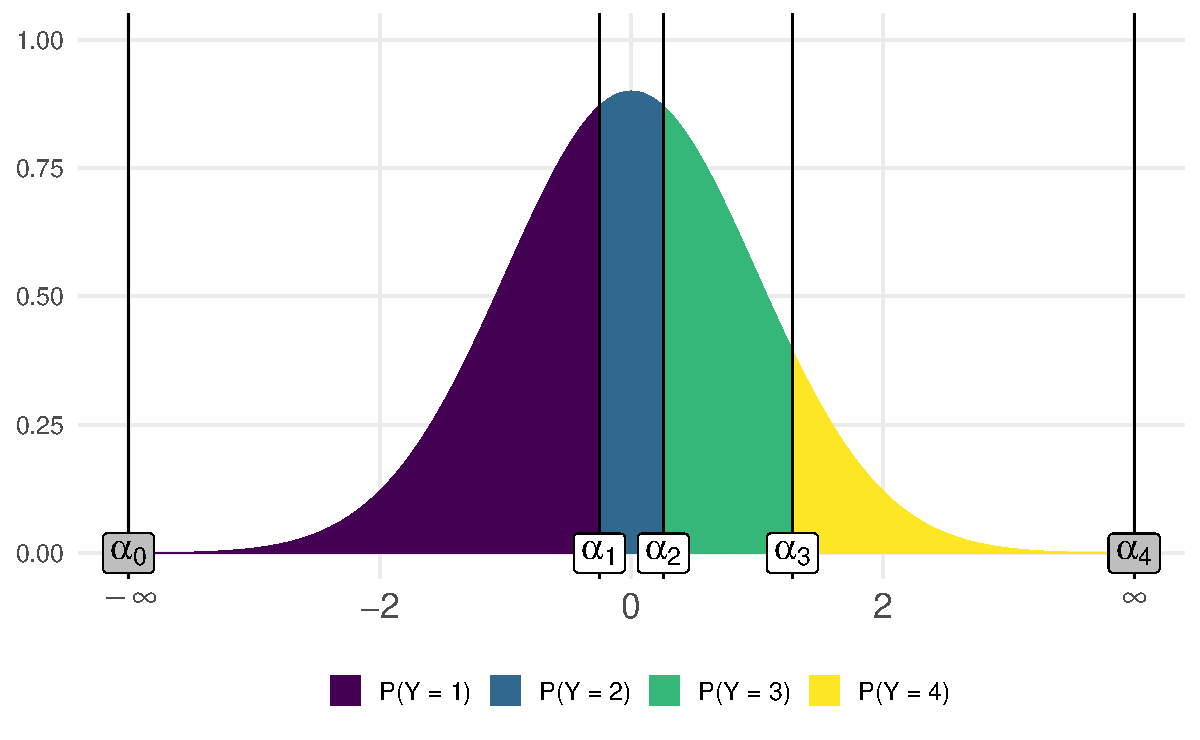
\includegraphics[width=1\linewidth]{paper_files/figure-latex/fig-explain-cumulative-1} 

}

\caption{Relationship between cumulative probabilities and ordinal outcomes. The \(Y^\star\) latent variable is segmented into \(k\) levels using \(k - 1\) thresholds (\(\alpha\)). The distance between thresholds determine the probability of each outcome. The grey thresholds are only used to compute the \(Y = 1\) and \(Y = k\) probabilities.}\label{fig:fig-explain-cumulative}
\end{figure}

\begin{center}\textbf{[Figure 1 about here]} \end{center}

\normalsize

Equation \eqref{eq:latent-model} shows the latent formulation of the previous model. The latent variable \(Y^\star\) is a function of the linear predictor \(\eta = \mathbf{X} \boldsymbol{\beta}\) similar to a standard regression.

\begin{equation}
\mathbf{Y^\star} = \mathbf{X}\boldsymbol{\beta} + \mathbf{\epsilon}
\label{eq:latent-model}
\end{equation}

The crucial part is \(\epsilon\) that is the random part (errors) of the model. For a \emph{probit} model, errors are sampled from a standard Normal distribution while for a \emph{logit} model from a standard logistic distribution. Following the notation by Tutz (2022), the observed ordinal value \(Y_i = k\) comes from \(Y^\star_i\) belonging to the interval defined by the thresholds \(Y_i = k \iff \alpha_{k - 1} < Y^\star_i < \alpha_{k}\) where \(- \infty = \alpha_0 < \alpha_1 < \dots< \alpha_{k - 1} < \alpha_k = \infty\).

The thresholds \(\alpha_k\) are considered fixed and part of the measurement procedure (Liddell \& Kruschke, 2018; see the \emph{location-shift} models by Tutz, 2022, where thresholds vary as a function of predictors). The model can be also formalized in alternative ways. Liddell and Kruschke (2018) and Kruschke (2015) proposed a Bayesian version of the model or Gelman, Hill, and Vehtari (2020) for other thresholds parametrizations.

The scale (spread) of the latent variable is fixed to one for both \emph{probit} and \emph{logit} models. In the supplementary materials we showed how to implement a location-scale models including predictors on the scale parameter (Cox, 1995; Rigby \& Stasinopoulos, 2005; Tutz, 2022).

\subsection{Link function}\label{link-function}

The CM implemented in Equations \eqref{eq:prob-cum-model1} and \eqref{eq:latent-model} requires specifying the link function \(g(\cdot)\) or the errors distribution \(\epsilon_i \sim D(\mu, \sigma^2)\) (\(D\) being a certain probability distribution). Among several available functions the \emph{logit} and \emph{probit} models are the most common. The \emph{logit} model use a \emph{logit} link function and a logistic distribution as latent variable. On the other side, the \emph{probit} model assume a latent Gaussian distribution using the inverse of the cumulative distribution (\(\Phi^{-1}\)) function as link function.

The two models provide similar results with a different parameters interpretation. In the next sections we will illustrate the differences and simulation strategies. Figure \ref{fig:fig-logit-vs-probit} depicts the two distributions while Table \ref{tab:tab-model-summary-latex} summarise the presented CM with the proposed link function and the corresponding R code.

In terms of parameters, both distributions can be defined with in terms of location \(\mu\) and scale \(s\). The standard normal distribution has \(\mu = 0\) and \(s = 1\). Furthermore the variance corresponds to the scale \(s^2 = \sigma^2 = 1\). The variance of the logistic distribution is \(\sigma^2 = \frac{s^2\pi^2}{3}\). The standard logistic distribution has \(\mu = 0\) and \(s^2 = 1\) thus the standard deviation simplified to \(\frac{\pi}{\sqrt{3}} \approx 1.81\). In practical terms, fixing \(\mu\) and \(s\) lead to an higher standard deviation for the logistic distribution.

\scriptsize

\begin{figure}

{\centering 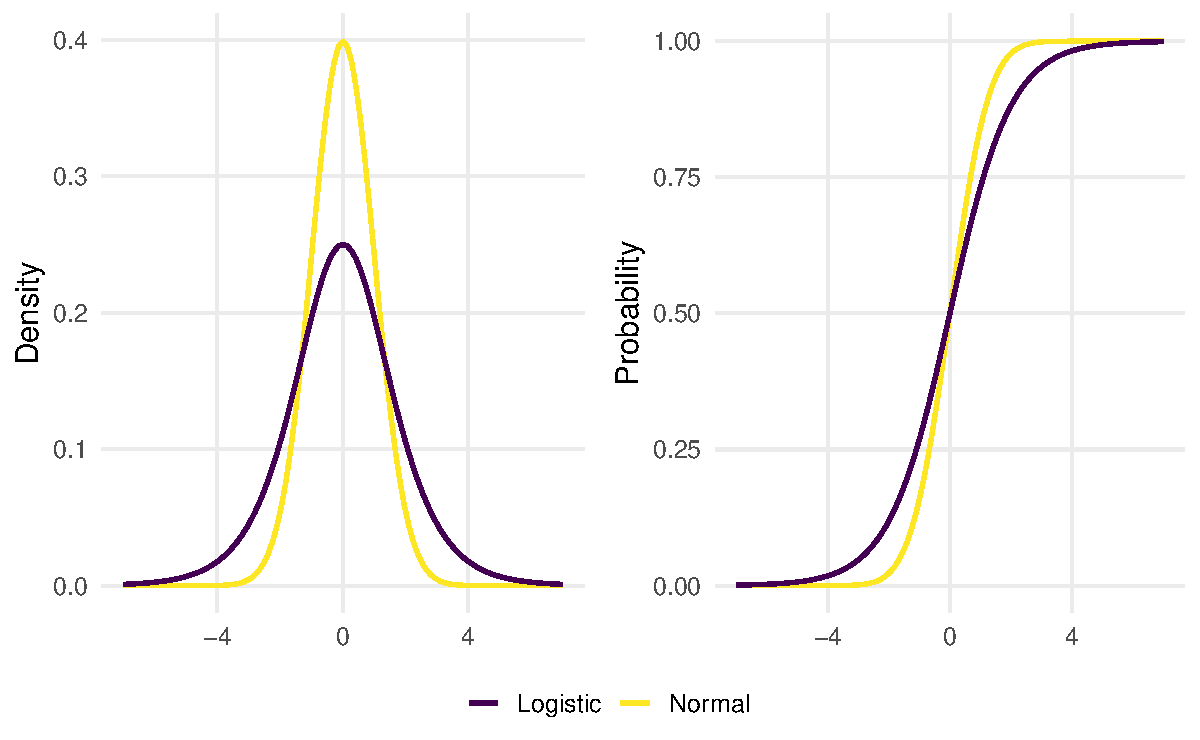
\includegraphics[width=1\linewidth]{paper_files/figure-latex/fig-logit-vs-probit-1} 

}

\caption{Difference between \emph{logit} and \emph{probit} models. On the left the probability density function (PDF). On the right the cumulative distribution function (CDF).}\label{fig:fig-logit-vs-probit}
\end{figure}

\begin{center}\textbf{[Figure 2 about here]} \end{center}

\normalsize

\scriptsize

\normalsize

\scriptsize

\begin{table}
\centering
\caption{\label{tab:tab-model-summary-latex}Summary of the probit and logit models in terms of link (\(g(\cdot)\)) and inverse link function (\(g^{-1}(\cdot)\)) and the corresponding R code.}
\centering
\begin{tabular}[t]{ccccc}
\toprule
\multicolumn{1}{c}{} & \multicolumn{2}{c}{Link Function $g(.)$} & \multicolumn{2}{c}{Inverse Link Function $g^{-1}(.)$} \\
\cmidrule(l{3pt}r{3pt}){2-3} \cmidrule(l{3pt}r{3pt}){4-5}
\textbf{Model} & \textbf{Equation} & \textbf{R Code} & \textbf{Equation} & \textbf{R Code}\\
\midrule
Cumulative Logit & $\text{logit}(p) = \text{log}(p / (1-p))$ & \texttt{qlogis()} & $e^{\text{logit}(p)} / (1 + e^{\text{logit}(p)})$ & \texttt{plogis()}\\
Cumulative Probit & $z = \Phi^{-1}(p)$ & \texttt{qnorm()} & $p = \Phi(z)$ & \texttt{pnorm()}\\
\bottomrule
\end{tabular}
\end{table}

\normalsize

\scriptsize

\normalsize

\section{Model fitting}\label{model-fitting}

For fitting the cumulative models we used the \texttt{ordinal} package (Christensen, 2019). Despite the presence of other possibilities the \texttt{ordinal} package provide the most complete and intuitive way to implement the ordinal models. The syntax is very similar to standard linear models in R and default functions to calculate predictions, perform model comparison, extract relevant model information are implemented similarly to standard regression modelling.\footnote{For a very complete overview of the ordinal package see Christensen (2019) and the Package documentation \url{https://cran.r-project.org/web/packages/ordinal/ordinal.pdf}}

The main function is \texttt{clm()} and the formula is specified using the syntax \texttt{y\ \textasciitilde{}\ ...} where \texttt{y} is the ordinal response and \texttt{...} is a combination of predictors. The package also implements mixed-effects models including random intercepts and slopes.

When fitting the model the crucial arguments are the \texttt{formula}, the \texttt{link} function and the \texttt{data}. More advanced arguments are the \texttt{nominal}, \texttt{scale} and \texttt{threshold}.

\begin{itemize}
\tightlist
\item
  \texttt{formula}: the formula \texttt{y\ \textasciitilde{}\ x} with the dependent variable and predictors.
\item
  \texttt{link}: is the link function. In this tutorial we consider only the \emph{logit} and \emph{probit} link but other link functions are available.
\item
  \texttt{data}: is the dataset with variables included in the \texttt{formula}
\item
  \texttt{nominal}: formula with predictors where the proportional odds assumption (See Section \ref{proportional-odds-assumption}) is relaxed (i.e., partial or non proportional odds)
\item
  \texttt{scale}: formula with predictors for the scale (standard deviation) parameter. This argument allow to fit a scale-location model (see supplementary materials). The main \texttt{formula} argument refers to predictors on the location parameter (i.e., the mean \(\mu\)).
\item
  \texttt{threshold}: different structures for estimating the thresholds. The default is \texttt{threshold\ =\ "flexible"} where \(k - 1\) threshold (where \(k\) is the number of ordinal levels for \(Y\)) are estimated.
\end{itemize}

We can start by fitting a simple model, highlighting the crucial parameters where the detailed explanation will be expanded in the next sections. Table \ref{tab:tab-dataset-example-latex} contains simulated data from \(n = 100\) participants rating the agreement about a certain item with \(k = 4\) ordered options. The participants are divided into two groups (\(x_a\) and \(x_b\)). We can fit a cumulative link model with \texttt{clm()} function and check the model summary.

\scriptsize

\normalsize

\scriptsize

\begin{table}
\centering
\caption{\label{tab:tab-dataset-example-latex}Summary of the simulated dataset. For each group (a and b) we reported mean, median and standard deviation of the ordinal outcome (metric descriptive statistics). For each ordinal outcome (\(Y\)) we reported the frequency and (within parentheses) the probability.}
\centering
\begin{tabular}[t]{cccccccc}
\toprule
\textbf{Group} & \textbf{Mean} & \textbf{Median} & \textbf{SD} & \textbf{Y1} & \textbf{Y2} & \textbf{Y3} & \textbf{Y4}\\
\midrule
a & 2.62 & 3 & 1.1 & \textbf{10} (p = \textit{0.2}) & \textbf{13} (p = \textit{0.26}) & \textbf{13} (p = \textit{0.26}) & \textbf{14} (p = \textit{0.28})\\
b & 3.06 & 3 & 1.04 & \textbf{6} (p = \textit{0.12}) & \textbf{7} (p = \textit{0.14}) & \textbf{15} (p = \textit{0.3}) & \textbf{22} (p = \textit{0.44})\\
\bottomrule
\end{tabular}
\end{table}

\normalsize

\scriptsize

\normalsize

\scriptsize

\begin{Shaded}
\begin{Highlighting}[]
\NormalTok{fit }\OtherTok{\textless{}{-}} \FunctionTok{clm}\NormalTok{(y }\SpecialCharTok{\textasciitilde{}}\NormalTok{ x, }\AttributeTok{data =}\NormalTok{ dat, }\AttributeTok{link =} \StringTok{"logit"}\NormalTok{)}
\FunctionTok{summary}\NormalTok{(fit)}
\CommentTok{\#\textgreater{} formula: y \textasciitilde{} x}
\CommentTok{\#\textgreater{} data:    dat}
\CommentTok{\#\textgreater{} }
\CommentTok{\#\textgreater{}  link  threshold nobs logLik  AIC    niter max.grad cond.H }
\CommentTok{\#\textgreater{}  logit flexible  100  {-}131.80 271.60 4(0)  2.13e{-}11 1.7e+01}
\CommentTok{\#\textgreater{} }
\CommentTok{\#\textgreater{} Coefficients:}
\CommentTok{\#\textgreater{}    Estimate Std. Error z value Pr(\textgreater{}|z|)  }
\CommentTok{\#\textgreater{} xb   0.7556     0.3685    2.05   0.0403 *}
\CommentTok{\#\textgreater{} {-}{-}{-}}
\CommentTok{\#\textgreater{} Signif. codes:  0 \textquotesingle{}***\textquotesingle{} 0.001 \textquotesingle{}**\textquotesingle{} 0.01 \textquotesingle{}*\textquotesingle{} 0.05 \textquotesingle{}.\textquotesingle{} 0.1 \textquotesingle{} \textquotesingle{} 1}
\CommentTok{\#\textgreater{} }
\CommentTok{\#\textgreater{} Threshold coefficients:}
\CommentTok{\#\textgreater{}     Estimate Std. Error z value}
\CommentTok{\#\textgreater{} 1|2  {-}1.3328     0.3126  {-}4.264}
\CommentTok{\#\textgreater{} 2|3  {-}0.2185     0.2703  {-}0.808}
\CommentTok{\#\textgreater{} 3|4   0.9767     0.2893   3.377}
\end{Highlighting}
\end{Shaded}

\normalsize

The two main sections of the model summary are the \emph{Coefficients} section reporting the regression coefficients \(\beta\) and the \emph{Threshold} section reporting the \(\alpha\) estimation. Given that \(k = 4\) we have \(k - 1 = 3\) thresholds and one \(\beta\) associated with the \(x\) effect. As in standard regression models, when \(x\) is a categorical predictor with \(j\) level, we will estimate \(j - 1\) regression coefficients (plus the intercept term) where the interpretation depends on the contrast coding (see Schad, Vasishth, Hohenstein, \& Kliegl, 2020). In R the default is the dummy coding where a factor of \(j\) levels is converted into \(j - 1\) dummy variables. By default, the first level of the factor is taken as the reference level and the \(j - 1\) coefficients represent the comparison between the other levels and the reference.

\section{Interpreting parameters}\label{interpreting-parameters}

\subsection{\texorpdfstring{\emph{Logit Model}. Odds and odds ratio}{Logit Model. Odds and odds ratio}}\label{logit-model.-odds-and-odds-ratio}

To understand the logit model we need to introduce odds and odds ratio. The odds of a probability \(p\) is defined as \(p/(1 - p)\) thus the success probability over the failure probability. The odds takes value ranging from \(0\) to \(\infty\). With a probability of \(p = 0.8\), we have odds of \(4\), indicating that there are four successes for each failure. The same as having \(p = 0.2\) and an odds of \(0.25\) means that for each \(0.25\) successes we have a failure (or \(4\) failures for each success). When comparing two groups or conditions we can take the ratio of two odds. An odds ratio (OR) of \(4\) means that the odds of success at the numerator is 4 times higher than the odds of success at the denominator. The Figure \ref{fig:fig-odds-example} shows the relationship between probabilities and odds. The logit transformation is about taking the logarithm of the odds creating a symmetric function ranging from \(-\infty\) to \(\infty\) with \(p = 0.5\) as the midpoint because \(\text{log}(0.5/(1 - 0.5)) = 0\).

\scriptsize

\begin{figure}

{\centering 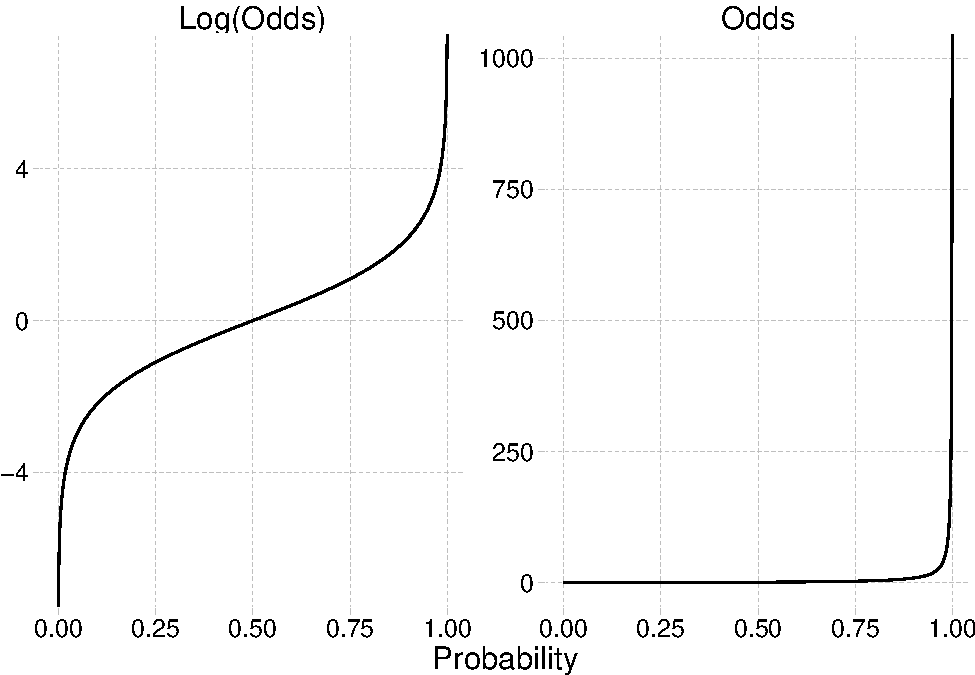
\includegraphics[width=1\linewidth]{paper_files/figure-latex/fig-odds-example-1} 

}

\caption{Relationship between probability (x axis) odds and the log odds. Using log odds ensure a symmetric relationship with a zero midpoint (\(p = 0.5\)).}\label{fig:fig-odds-example}
\end{figure}

\begin{center}\textbf{[Figure 3 about here]} \end{center}

\normalsize

Odds and odds ratios are clearly defined with \(k = 2\) outcomes. With an ordinal variable and a cumulative model we can use the cumulative odds ratio. With e.g.~\(k = 4\) outcomes we have \(k - 1\) odds ratios determined by the cumulative probability in terms of \(P(Y \leq 1), \dots, P(Y \leq k - 1)\) comparing the two groups.

For example the probability of responding \(Y \leq 1\) in the group ``a'' is 0.20 corresponding to an odds of 0.25. When calculating the odds ratio comparing ``a'' vs ``b'' for \(Y \leq 1\) we obtain that the group ``a'' has 1.83 times the odds of responding \(Y \leq 1\) compared to the group ``b''.

\scriptsize

\begin{Shaded}
\begin{Highlighting}[]
\CommentTok{\# function to calculate odds}
\NormalTok{odds }\OtherTok{\textless{}{-}} \ControlFlowTok{function}\NormalTok{(p) p }\SpecialCharTok{/}\NormalTok{ (}\DecValTok{1} \SpecialCharTok{{-}}\NormalTok{ p)}

\CommentTok{\# the dummy\_ord() is a custom function creating k {-} 1 dummy variable for the cumulative probabilities}

\CommentTok{\# data.frame with the group (x) and the k {-} 1 dummy variables}
\NormalTok{cum\_p }\OtherTok{\textless{}{-}} \FunctionTok{cbind}\NormalTok{(}\AttributeTok{x =}\NormalTok{ dat}\SpecialCharTok{$}\NormalTok{x, }\FunctionTok{dummy\_ord}\NormalTok{(dat}\SpecialCharTok{$}\NormalTok{y))}

\CommentTok{\# calculating the cumulative probability for k {-} 1 variables. }
\CommentTok{\# Taking the average of a series of 0{-}1 is the same as computing the proportion of 1s.}
\NormalTok{(group\_a }\OtherTok{\textless{}{-}} \FunctionTok{apply}\NormalTok{(cum\_p[cum\_p}\SpecialCharTok{$}\NormalTok{x }\SpecialCharTok{==} \StringTok{"a"}\NormalTok{, }\SpecialCharTok{{-}}\DecValTok{1}\NormalTok{], }\DecValTok{2}\NormalTok{, mean))}
\CommentTok{\#\textgreater{} y1vs234 y12vs34 y123vs4 }
\CommentTok{\#\textgreater{}    0.20    0.46    0.72}
\NormalTok{(group\_b }\OtherTok{\textless{}{-}} \FunctionTok{apply}\NormalTok{(cum\_p[cum\_p}\SpecialCharTok{$}\NormalTok{x }\SpecialCharTok{==} \StringTok{"b"}\NormalTok{, }\SpecialCharTok{{-}}\DecValTok{1}\NormalTok{], }\DecValTok{2}\NormalTok{, mean))}
\CommentTok{\#\textgreater{} y1vs234 y12vs34 y123vs4 }
\CommentTok{\#\textgreater{}    0.12    0.26    0.56}

\CommentTok{\# calculating k {-} 1 odds ratios on the cumulative probabilities as a/b}
\FunctionTok{odds}\NormalTok{(group\_a) }\SpecialCharTok{/} \FunctionTok{odds}\NormalTok{(group\_b)}
\CommentTok{\#\textgreater{}  y1vs234  y12vs34  y123vs4 }
\CommentTok{\#\textgreater{} 1.833333 2.424501 2.020408}
\end{Highlighting}
\end{Shaded}

\normalsize

\subsection{Proportional odds assumption}\label{proportional-odds-assumption}

Following again the taxonomy by Tutz (2022), each of the presented ordinal regression model has a basic version making the PO assumption. There are more advanced versions of the model relaxing this assumption completely (\emph{non proportional odds}) and partially (\emph{partial proportional odds}, Peterson \& Harrell, 1990).

When fitting a logit model, the coefficients \(\beta_j\) are the (log) odds ratios for a unit increase in \(x\). However, the previous model estimate a single \(\beta\) even if we have four ordinal outcomes. The CM model (in the basic version) made an assumption called \emph{proportional odds} (PO). Under this assumption we assume that the \(k - 1\) cumulative odds ratios are the same. The PO assumption is formalized in Equation \eqref{eq:prop-odds}. The cumulative log odds ratio comparing \(P(Y_k|x_0)\) with \(P(Y_k|x_1)\) is the same regardless the specific threshold (\(\beta_1 = \beta_2 \dots = \beta_{k - 1}\)). The Figure (\ref{fig:fig-prop-odds}) depicts the proportional odds assumption for the \(k - 1\) logistic curves both for probabilities and linear predictors \(\eta\).

\begin{equation}
\text{logit} (\frac{P(Y \leq 1 |x_1)}{P(Y \leq 1 |x_0)}) = \dots = \text{logit} (\frac{P(Y \leq k - 1 |x_1)}{P(Y \leq k -1 |x_0)})
\label{eq:prop-odds}
\end{equation}

\scriptsize

\begin{figure}

{\centering 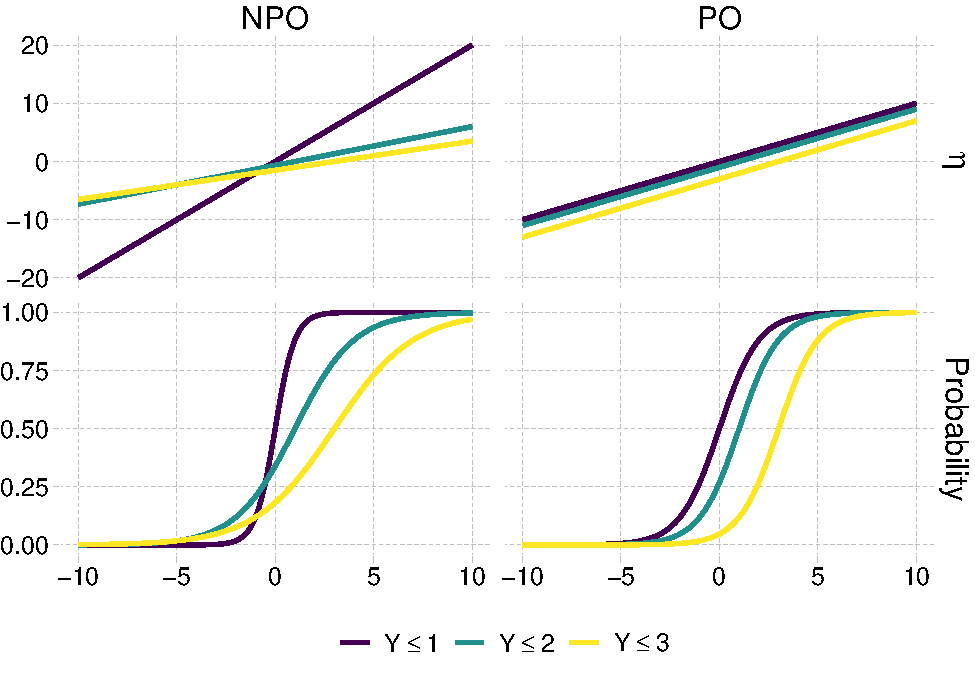
\includegraphics[width=1\linewidth]{paper_files/figure-latex/fig-prop-odds-1} 

}

\caption{Example of proportional odds (PO, right) and non-proportional odds (NPO, left) for cumulative probabilities and the linear predictor \(\eta\) assuming a continuous predictor \(x\). Data supporting the PO assumption shows an horizontal shift in the cumulative probability with the same slope while for NPO model slopes can be heterogeneous.}\label{fig:fig-prop-odds}
\end{figure}

\begin{center}\textbf{[Figure 4 about here]} \end{center}

\normalsize

There are CM models relaxing this assumption completely (\emph{non proportional odds}, Tutz, 2022) or partially (\emph{partial proportional odds}, Peterson \& Harrell, 1990). The PO model is more parsimonious but the PO assumption could be considered too strict. There are several methods for testing if data are supporting the PO assumption (see Liu, He, Tu, \& Tang, 2023 for an overview). Tutz and Berger (2020) suggested a trade-off between assuming/relaxing the PO assumption by fitting \emph{location-shift} or \emph{location-scale} models. Basically these methods should guarantee more flexibility in modelling the observed probabilities reducing the number of parameters. However, these methods and models are outside the scope of the tutorial.

In the previous code block, we estimated the \(k - 1\) odds ratios and they were different even if data have been simulated under the PO assumption (see the Simulating data section). Calculating the odds ratios using predicted probabilities from the model fitted with \texttt{clm()} (that by default assume the PO) the odds ratios are the same. In the following code block we computed the odds ratio comparing \(x_a\) and \(x_b\) when \(k \leq 1\) and \(k \leq 2\).

\scriptsize

\begin{Shaded}
\begin{Highlighting}[]
\CommentTok{\# fitting the model}
\NormalTok{fit }\OtherTok{\textless{}{-}} \FunctionTok{clm}\NormalTok{(y }\SpecialCharTok{\textasciitilde{}}\NormalTok{ x, }\AttributeTok{data =}\NormalTok{ dat, }\AttributeTok{link =} \StringTok{"logit"}\NormalTok{)}

\CommentTok{\# extracting the predicted probabilities for the two groups}
\NormalTok{pr }\OtherTok{\textless{}{-}} \FunctionTok{predict}\NormalTok{(fit, }\FunctionTok{data.frame}\NormalTok{(}\AttributeTok{x =} \FunctionTok{unique}\NormalTok{(dat}\SpecialCharTok{$}\NormalTok{x)))}\SpecialCharTok{$}\NormalTok{fit}

\CommentTok{\# y \textless{}= 1}
\NormalTok{y1a }\OtherTok{\textless{}{-}}\NormalTok{ pr[}\DecValTok{1}\NormalTok{, }\DecValTok{1}\NormalTok{]}
\NormalTok{y1b }\OtherTok{\textless{}{-}}\NormalTok{ pr[}\DecValTok{2}\NormalTok{, }\DecValTok{1}\NormalTok{]}

\CommentTok{\# y \textless{}= 2}
\NormalTok{y12a }\OtherTok{\textless{}{-}} \FunctionTok{sum}\NormalTok{(pr[}\DecValTok{1}\NormalTok{, }\DecValTok{1}\SpecialCharTok{:}\DecValTok{2}\NormalTok{])}
\NormalTok{y12b }\OtherTok{\textless{}{-}} \FunctionTok{sum}\NormalTok{(pr[}\DecValTok{2}\NormalTok{, }\DecValTok{1}\SpecialCharTok{:}\DecValTok{2}\NormalTok{])}

\CommentTok{\# odds ratio y \textless{}= 1 (a vs b) VS y \textless{}= 2 (a vs b)}
\FunctionTok{odds}\NormalTok{(y1a) }\SpecialCharTok{/} \FunctionTok{odds}\NormalTok{(y1b)}
\CommentTok{\#\textgreater{} [1] 2.128857}
\FunctionTok{odds}\NormalTok{(y12a) }\SpecialCharTok{/} \FunctionTok{odds}\NormalTok{(y12b)}
\CommentTok{\#\textgreater{} [1] 2.128857}
\end{Highlighting}
\end{Shaded}

\normalsize

\subsection{\texorpdfstring{\emph{Probit Model} and \(\mathbf{z}\) scores}{Probit Model and \textbackslash mathbf\{z\} scores}}\label{probit-model-and-mathbfz-scores}

When assuming a standard Gaussian distribution we are fitting \emph{probit} model. The main difference regards the parameters interpretation. In the logit model the \(\boldsymbol{\beta}\) are the log odds ratio. For categorical variables they represents the increase in the log odds of moving from one level to the other while for numerical variables is the increase in the log odds for a unit increase in \(x\).

For the \emph{probit} model, the \(\beta\) is the increase in terms of \(z\) scores for a unit increase in \(x\). This is very convenient especially for categorical variables because parameters can be interpreted as a Cohen's \(d\) like measure. Thinking about the latent distributions, the \(\beta\) is the shift in the latent mean comparing two or more groups or the slope of latent scores as a function of a numeric \(x\). More formally the shift in the latent distribution is \(\beta/\sigma\) (for the \emph{probit} model \(\sigma = 1\)). The interpretation in terms of shifting the latent mean holds also for the logistic model. However, the standard deviation of the standard logistic regression is \(\frac{\pi}{\sqrt{3}} \approx 1.81\)\footnote{Actually the variance of the logistic distribution is \(\frac{s^2\pi^2}{3}\) and the standard deviation \(\frac{s\pi}{\sqrt{3}}\) where \(s\) is the scale of the distribution. For the standard logistic distribution \(s = 1\) (as for the standard normal distribution).}. The \(\beta\) for the logistic distribution can be interpreted as the location shift of the latent logistic distribution by \(\beta/(\frac{\pi}{\sqrt{3}})\) standard deviations (Agresti, 2010).

\subsubsection{\texorpdfstring{Proportional odds and \emph{probit} model}{Proportional odds and probit model}}\label{proportional-odds-and-probit-model}

The PO assumption is relevant only for the \emph{logit} model. When using the \emph{probit} link function we can use the terms \emph{parallel slopes} for the assumption of a common \(\beta\) (see Equation \eqref{eq:probit-prop-odds}). In practical terms, difference in \(z\) scores for a unit increase in \(x\) (the actual interpretation of \(\beta\) in a \emph{probit} model) is the same regardless of the threshold. As for the previous example, we can fit the \emph{probit} model and manually calculate the difference in \(z\) scores.

\begin{equation}
z_{x_1 - x_0} = \Phi(P \leq 1|x_1) - \Phi(P \leq 1|x_0) = \dots = \Phi(P \leq k - 1|x_1) - \Phi(P \leq k - 1|x_0)
\label{eq:probit-prop-odds}
\end{equation}

\scriptsize

\begin{Shaded}
\begin{Highlighting}[]
\CommentTok{\# fitting the model}
\NormalTok{fit }\OtherTok{\textless{}{-}} \FunctionTok{clm}\NormalTok{(y }\SpecialCharTok{\textasciitilde{}}\NormalTok{ x, }\AttributeTok{data =}\NormalTok{ dat, }\AttributeTok{link =} \StringTok{"probit"}\NormalTok{)}

\CommentTok{\# extracting the predicted probabilities for the two groups}
\NormalTok{pr }\OtherTok{\textless{}{-}} \FunctionTok{predict}\NormalTok{(fit, }\FunctionTok{data.frame}\NormalTok{(}\AttributeTok{x =} \FunctionTok{unique}\NormalTok{(dat}\SpecialCharTok{$}\NormalTok{x)))}\SpecialCharTok{$}\NormalTok{fit}

\CommentTok{\# y \textless{}= 1}
\NormalTok{y1a }\OtherTok{\textless{}{-}}\NormalTok{ pr[}\DecValTok{1}\NormalTok{, }\DecValTok{1}\NormalTok{]}
\NormalTok{y1b }\OtherTok{\textless{}{-}}\NormalTok{ pr[}\DecValTok{2}\NormalTok{, }\DecValTok{1}\NormalTok{]}

\CommentTok{\# y \textless{}= 2}
\NormalTok{y12a }\OtherTok{\textless{}{-}} \FunctionTok{sum}\NormalTok{(pr[}\DecValTok{1}\NormalTok{, }\DecValTok{1}\SpecialCharTok{:}\DecValTok{2}\NormalTok{])}
\NormalTok{y12b }\OtherTok{\textless{}{-}} \FunctionTok{sum}\NormalTok{(pr[}\DecValTok{2}\NormalTok{, }\DecValTok{1}\SpecialCharTok{:}\DecValTok{2}\NormalTok{])}

\CommentTok{\# z score difference y \textless{}= 1 (a vs b) VS y \textless{}= 2 (a vs b)}
\FunctionTok{qnorm}\NormalTok{(y1a) }\SpecialCharTok{{-}} \FunctionTok{qnorm}\NormalTok{(y1b)}
\CommentTok{\#\textgreater{} [1] 0.4408949}
\FunctionTok{qnorm}\NormalTok{(y12a) }\SpecialCharTok{{-}} \FunctionTok{qnorm}\NormalTok{(y12b)}
\CommentTok{\#\textgreater{} [1] 0.4408949}
\end{Highlighting}
\end{Shaded}

\normalsize

\subsection{Simulating data}\label{simulating-data}

In this tutorial we present two method for simulating ordinal data. Simulating data is a powerful strategy to understand the model (DeBruine \& Barr, 2021) and estimate statistical properties (e.g., power or type-1 error). The first simulation method calculate the probabilities of each \(Y\) level as a function of predictors and generate data from a \emph{multinomial} distribution. The second method simulate data using the the latent formulation. Whenever random number generation occurs, it is appropriate to set a \texttt{seed} (\texttt{set.seed()} function, in this case we use \texttt{set.seed(2024)}). Running again the same code will produce the same result. A general simulation approach concerns generating a dataset from the assumed data generation process, fitting the statistical model and assessing the recovery of simulated parameters. To check the simulation approach, using a large sample size produce estimations with small sampling error. A limited sample size even when fitting the true model will produce variable estimations.

\subsubsection{Simulating from a multinomial distribution}\label{simulating-from-a-multinomial-distribution}

For the first method we need to calculate \(g^{-1}(\eta)\) as a function of predictors and then sample from a \emph{multinomial} (more specifically \emph{categorical}) distribution using the \texttt{sample()} function in R. This method is similar to the general way of simulating data for a generalized linear model (see the supplementary materials for a general overview).

As a simple example, let's simulate two groups with \(n = 100\) participants responding to an item (\(Y\)) with \(k = 4\) ordered options. We simulate the second group having higher probability of responding higher categories of \(Y\).

As explained in the previous sections, we can summarise the effect size of a CM (assuming PO) using a single \(\beta = \log(OR)\). We can assume that the odds ratio is \(OR = 2\). For simplicity, the probabilities of the first group \(x = 0\) are uniform thus \(P(Y = 1|x_0) = \dots P(Y = k|x_0) = 1/k\). The following code summarise the first steps of the simulation. Basically we define the simulation parameters, we calculate the \(k - 1\) thresholds \(\alpha\) and we apply Equations \eqref{eq:prob-cum-model1} and \eqref{eq:prob-cum-model2}. In this way we calculated the true probability of each \(Y\) level for the two groups.

An important step is converting from \(\alpha\) to probabilities or the opposite. This steps are implemented in the \texttt{alpha\_to\_prob()} and \texttt{prob\_to\_alpha()} functions that given the input return thresholds or probabilities.

\scriptsize

\begin{Shaded}
\begin{Highlighting}[]
\NormalTok{k }\OtherTok{\textless{}{-}} \DecValTok{5}
\NormalTok{(p }\OtherTok{\textless{}{-}} \FunctionTok{rep}\NormalTok{(}\DecValTok{1}\SpecialCharTok{/}\NormalTok{k, k)) }\CommentTok{\# uniform}
\CommentTok{\#\textgreater{} [1] 0.2 0.2 0.2 0.2 0.2}
\FunctionTok{names}\NormalTok{(p) }\OtherTok{\textless{}{-}} \FunctionTok{paste0}\NormalTok{(}\StringTok{"y"}\NormalTok{, }\DecValTok{1}\SpecialCharTok{:}\NormalTok{k)}

\NormalTok{(alpha }\OtherTok{\textless{}{-}} \FunctionTok{prob\_to\_alpha}\NormalTok{(p, }\AttributeTok{link =} \StringTok{"logit"}\NormalTok{)) }\CommentTok{\# or prob\_to\_alpha(p, "probit")}
\CommentTok{\#\textgreater{}        1|2        2|3        3|4        4|5 }
\CommentTok{\#\textgreater{} {-}1.3862944 {-}0.4054651  0.4054651  1.3862944}
\FunctionTok{alpha\_to\_prob}\NormalTok{(alpha, }\AttributeTok{link =} \StringTok{"logit"}\NormalTok{)}
\CommentTok{\#\textgreater{}  p1  p2  p3  p4  p5 }
\CommentTok{\#\textgreater{} 0.2 0.2 0.2 0.2 0.2}
\end{Highlighting}
\end{Shaded}

\normalsize

\scriptsize

\begin{Shaded}
\begin{Highlighting}[]
\DocumentationTok{\#\# SIMULATION PARAMETERS}

\NormalTok{N }\OtherTok{\textless{}{-}} \DecValTok{100} \CommentTok{\# sample size}
\NormalTok{or }\OtherTok{\textless{}{-}} \DecValTok{2} \CommentTok{\# odds ratio}
\NormalTok{k }\OtherTok{\textless{}{-}} \DecValTok{4} \CommentTok{\# number of ordinal alternatives}
\NormalTok{prob0 }\OtherTok{\textless{}{-}} \FunctionTok{rep}\NormalTok{(}\DecValTok{1}\SpecialCharTok{/}\NormalTok{k, k) }\CommentTok{\# probabilities for the first group}
\NormalTok{alpha }\OtherTok{\textless{}{-}} \FunctionTok{prob\_to\_alpha}\NormalTok{(prob0, }\AttributeTok{link =} \StringTok{"logit"}\NormalTok{)}
\NormalTok{dat }\OtherTok{\textless{}{-}} \FunctionTok{data.frame}\NormalTok{(}\AttributeTok{x =} \FunctionTok{rep}\NormalTok{(}\FunctionTok{c}\NormalTok{(}\DecValTok{0}\NormalTok{, }\DecValTok{1}\NormalTok{), }\AttributeTok{each =}\NormalTok{ N}\SpecialCharTok{/}\DecValTok{2}\NormalTok{))}

\DocumentationTok{\#\# LINEAR PREDICTOR}

\CommentTok{\# calculate linear predictor using equation 1 obtaining k {-} 1 equations}

\NormalTok{lp }\OtherTok{\textless{}{-}} \FunctionTok{lapply}\NormalTok{(alpha, }\ControlFlowTok{function}\NormalTok{(a) a }\SpecialCharTok{{-}} \FunctionTok{log}\NormalTok{(or) }\SpecialCharTok{*}\NormalTok{ dat}\SpecialCharTok{$}\NormalTok{x)}
\FunctionTok{names}\NormalTok{(lp) }\OtherTok{\textless{}{-}} \FunctionTok{sprintf}\NormalTok{(}\StringTok{"lp\_leq\%s"}\NormalTok{, }\DecValTok{1}\SpecialCharTok{:}\NormalTok{(k }\SpecialCharTok{{-}} \DecValTok{1}\NormalTok{)) }\CommentTok{\# giving appropriate names}
\NormalTok{lp }\OtherTok{\textless{}{-}} \FunctionTok{data.frame}\NormalTok{(lp)}
\FunctionTok{head}\NormalTok{(lp)}
\CommentTok{\#\textgreater{}     lp\_leq1 lp\_leq2  lp\_leq3}
\CommentTok{\#\textgreater{} 1 {-}1.098612       0 1.098612}
\CommentTok{\#\textgreater{} 2 {-}1.098612       0 1.098612}
\CommentTok{\#\textgreater{} 3 {-}1.098612       0 1.098612}
\CommentTok{\#\textgreater{} 4 {-}1.098612       0 1.098612}
\CommentTok{\#\textgreater{} 5 {-}1.098612       0 1.098612}
\CommentTok{\#\textgreater{} 6 {-}1.098612       0 1.098612}

\DocumentationTok{\#\# CUMULATIVE PROBABILITIES}

\CommentTok{\# apply the inverse of the link function (invlogit) to calculate cumulative probabilities}
\NormalTok{cump }\OtherTok{\textless{}{-}} \FunctionTok{lapply}\NormalTok{(lp, plogis)}
\NormalTok{cump }\OtherTok{\textless{}{-}} \FunctionTok{data.frame}\NormalTok{(cump)}
\FunctionTok{names}\NormalTok{(cump) }\OtherTok{\textless{}{-}} \FunctionTok{sprintf}\NormalTok{(}\StringTok{"cump\_leq\%s"}\NormalTok{, }\DecValTok{1}\SpecialCharTok{:}\NormalTok{(k }\SpecialCharTok{{-}} \DecValTok{1}\NormalTok{)) }\CommentTok{\# giving appropriate names}
\FunctionTok{head}\NormalTok{(cump)}
\CommentTok{\#\textgreater{}   cump\_leq1 cump\_leq2 cump\_leq3}
\CommentTok{\#\textgreater{} 1      0.25       0.5      0.75}
\CommentTok{\#\textgreater{} 2      0.25       0.5      0.75}
\CommentTok{\#\textgreater{} 3      0.25       0.5      0.75}
\CommentTok{\#\textgreater{} 4      0.25       0.5      0.75}
\CommentTok{\#\textgreater{} 5      0.25       0.5      0.75}
\CommentTok{\#\textgreater{} 6      0.25       0.5      0.75}

\DocumentationTok{\#\# PROBABILITIES OF Y}

\CommentTok{\# for each row, we can calculate P(Y = k) using equation 2}
\CommentTok{\# P(Y = 1) = P(Y \textless{}= 1)}
\CommentTok{\# P(Y = 2) = P(Y \textless{}= 2) {-} P(Y \textless{}= 1)}
\CommentTok{\# P(Y = 3) = P(Y \textless{}= 3) {-} P(Y \textless{}= 2)}
\CommentTok{\# P(Y = 4) = 1 {-} P(Y \textless{}= 3)}

\CommentTok{\# adding a columns of 0 and 1, then diff() for adjacent differences}
\NormalTok{cump }\OtherTok{\textless{}{-}} \FunctionTok{cbind}\NormalTok{(}\DecValTok{0}\NormalTok{, cump, }\DecValTok{1}\NormalTok{)}
\NormalTok{p }\OtherTok{\textless{}{-}} \FunctionTok{apply}\NormalTok{(cump, }\DecValTok{1}\NormalTok{, diff, }\AttributeTok{simplify =} \ConstantTok{FALSE}\NormalTok{)}

\NormalTok{p }\OtherTok{\textless{}{-}} \FunctionTok{data.frame}\NormalTok{(}\FunctionTok{do.call}\NormalTok{(rbind, p)) }\CommentTok{\# collapse list of rows into a dataframe}
\FunctionTok{names}\NormalTok{(p) }\OtherTok{\textless{}{-}} \FunctionTok{sprintf}\NormalTok{(}\StringTok{"p\%s"}\NormalTok{, }\DecValTok{1}\SpecialCharTok{:}\NormalTok{k) }\CommentTok{\# giving appropriate names}
\FunctionTok{head}\NormalTok{(p)}
\CommentTok{\#\textgreater{}     p1   p2   p3   p4}
\CommentTok{\#\textgreater{} 1 0.25 0.25 0.25 0.25}
\CommentTok{\#\textgreater{} 2 0.25 0.25 0.25 0.25}
\CommentTok{\#\textgreater{} 3 0.25 0.25 0.25 0.25}
\CommentTok{\#\textgreater{} 4 0.25 0.25 0.25 0.25}
\CommentTok{\#\textgreater{} 5 0.25 0.25 0.25 0.25}
\CommentTok{\#\textgreater{} 6 0.25 0.25 0.25 0.25}

\CommentTok{\# probabilities for id = 1 (x = 0) and id = 51 (x = 1)}
\NormalTok{p[}\FunctionTok{c}\NormalTok{(}\DecValTok{1}\NormalTok{, }\DecValTok{51}\NormalTok{), ]}
\CommentTok{\#\textgreater{}           p1        p2        p3   p4}
\CommentTok{\#\textgreater{} 1  0.2500000 0.2500000 0.2500000 0.25}
\CommentTok{\#\textgreater{} 51 0.1428571 0.1904762 0.2666667 0.40}

\DocumentationTok{\#\# CUMULATIVE ODDS RATIO}

\CommentTok{\# calculate the (cumulative) odds ratio}

\NormalTok{x0 }\OtherTok{\textless{}{-}}\NormalTok{ cump[}\DecValTok{1}\NormalTok{, }\DecValTok{2}\SpecialCharTok{:}\NormalTok{k]}
\NormalTok{x1 }\OtherTok{\textless{}{-}}\NormalTok{ cump[}\DecValTok{51}\NormalTok{, }\DecValTok{2}\SpecialCharTok{:}\NormalTok{k]}

\CommentTok{\# this is the same as the or (the b1) and we are assuming POA}
\FunctionTok{odds}\NormalTok{(x0) }\SpecialCharTok{/} \FunctionTok{odds}\NormalTok{(x1)}
\CommentTok{\#\textgreater{}   cump\_leq1 cump\_leq2 cump\_leq3}
\CommentTok{\#\textgreater{} 1         2         2         2}
\end{Highlighting}
\end{Shaded}

\normalsize

\scriptsize

\begin{Shaded}
\begin{Highlighting}[]

\DocumentationTok{\#\# SAMPLING FROM THE MULTINOMIAL DISTRIBUTION}

\FunctionTok{set.seed}\NormalTok{(}\DecValTok{2024}\NormalTok{)}

\CommentTok{\# example of a random Y outcome based on the probabilities}
\FunctionTok{sample}\NormalTok{(}\AttributeTok{x =} \DecValTok{1}\SpecialCharTok{:}\NormalTok{k, }\AttributeTok{size =} \DecValTok{1}\NormalTok{, }\AttributeTok{prob =}\NormalTok{ p[}\DecValTok{1}\NormalTok{, ])}
\CommentTok{\#\textgreater{} [1] 1}

\CommentTok{\# we can apply it to the full dataset, this step lead to different results}
\CommentTok{\# each time we run the code because we are sampling from a distribution}

\NormalTok{dat}\SpecialCharTok{$}\NormalTok{y }\OtherTok{\textless{}{-}} \FunctionTok{apply}\NormalTok{(p, }\DecValTok{1}\NormalTok{, }\ControlFlowTok{function}\NormalTok{(ps) }\FunctionTok{sample}\NormalTok{(}\DecValTok{1}\SpecialCharTok{:}\NormalTok{k, }\AttributeTok{size =} \DecValTok{1}\NormalTok{, }\AttributeTok{prob =}\NormalTok{ ps))}
\FunctionTok{head}\NormalTok{(dat)}
\CommentTok{\#\textgreater{}   x y}
\CommentTok{\#\textgreater{} 1 0 3}
\CommentTok{\#\textgreater{} 2 0 4}
\CommentTok{\#\textgreater{} 3 0 4}
\CommentTok{\#\textgreater{} 4 0 3}
\CommentTok{\#\textgreater{} 5 0 4}
\CommentTok{\#\textgreater{} 6 0 3}

\CommentTok{\# let\textquotesingle{}s compute the observed probabilities, to be compared to the true}
\CommentTok{\# probabilities}

\CommentTok{\# observed}
\NormalTok{(op }\OtherTok{\textless{}{-}} \FunctionTok{prop.table}\NormalTok{(}\FunctionTok{table}\NormalTok{(dat}\SpecialCharTok{$}\NormalTok{x, dat}\SpecialCharTok{$}\NormalTok{y), }\AttributeTok{margin =} \DecValTok{1}\NormalTok{))}
\CommentTok{\#\textgreater{}    }
\CommentTok{\#\textgreater{}        1    2    3    4}
\CommentTok{\#\textgreater{}   0 0.26 0.22 0.26 0.26}
\CommentTok{\#\textgreater{}   1 0.10 0.18 0.30 0.42}

\CommentTok{\# true (just selecting a row from x = 0 and x = 1)}
\NormalTok{p[}\FunctionTok{c}\NormalTok{(}\DecValTok{1}\NormalTok{, }\DecValTok{51}\NormalTok{), ]}
\CommentTok{\#\textgreater{}           p1        p2        p3   p4}
\CommentTok{\#\textgreater{} 1  0.2500000 0.2500000 0.2500000 0.25}
\CommentTok{\#\textgreater{} 51 0.1428571 0.1904762 0.2666667 0.40}

\CommentTok{\# similarly we can compute the observed cumulative odds ratios}

\NormalTok{(cum\_op }\OtherTok{\textless{}{-}} \FunctionTok{apply}\NormalTok{(op, }\DecValTok{1}\NormalTok{, cumsum))}
\CommentTok{\#\textgreater{}    }
\CommentTok{\#\textgreater{}        0    1}
\CommentTok{\#\textgreater{}   1 0.26 0.10}
\CommentTok{\#\textgreater{}   2 0.48 0.28}
\CommentTok{\#\textgreater{}   3 0.74 0.58}
\CommentTok{\#\textgreater{}   4 1.00 1.00}
\FunctionTok{odds}\NormalTok{(cum\_op[}\SpecialCharTok{{-}}\NormalTok{k, }\DecValTok{1}\NormalTok{]) }\SpecialCharTok{/} \FunctionTok{odds}\NormalTok{(cum\_op[}\SpecialCharTok{{-}}\NormalTok{k, }\DecValTok{2}\NormalTok{]) }\CommentTok{\# {-}k remove the P(y = k) = 1}
\CommentTok{\#\textgreater{}        1        2        3 }
\CommentTok{\#\textgreater{} 3.162162 2.373626 2.061008}
 
\CommentTok{\# the odds ratios are not the same as the parameter. as we increase N}
\CommentTok{\# the parameter will converge to the true value}
\end{Highlighting}
\end{Shaded}

\normalsize

\scriptsize

\begin{Shaded}
\begin{Highlighting}[]
\NormalTok{dat}\SpecialCharTok{$}\NormalTok{y }\OtherTok{\textless{}{-}} \FunctionTok{ordered}\NormalTok{(dat}\SpecialCharTok{$}\NormalTok{y) }\CommentTok{\# make an ordered factor in R where 1 \textless{} 2 \textless{} 3 \textless{} 4}
\NormalTok{fit }\OtherTok{\textless{}{-}} \FunctionTok{clm}\NormalTok{(y }\SpecialCharTok{\textasciitilde{}}\NormalTok{ x, }\AttributeTok{data =}\NormalTok{ dat, }\AttributeTok{link =} \StringTok{"probit"}\NormalTok{)}
\FunctionTok{summary}\NormalTok{(fit)}
\CommentTok{\#\textgreater{} formula: y \textasciitilde{} x}
\CommentTok{\#\textgreater{} data:    dat}
\CommentTok{\#\textgreater{} }
\CommentTok{\#\textgreater{}  link   threshold nobs logLik  AIC    niter max.grad cond.H }
\CommentTok{\#\textgreater{}  probit flexible  100  {-}132.59 273.17 5(0)  2.86e{-}09 1.7e+01}
\CommentTok{\#\textgreater{} }
\CommentTok{\#\textgreater{} Coefficients:}
\CommentTok{\#\textgreater{}   Estimate Std. Error z value Pr(\textgreater{}|z|)  }
\CommentTok{\#\textgreater{} x   0.5183     0.2197   2.359   0.0183 *}
\CommentTok{\#\textgreater{} {-}{-}{-}}
\CommentTok{\#\textgreater{} Signif. codes:  0 \textquotesingle{}***\textquotesingle{} 0.001 \textquotesingle{}**\textquotesingle{} 0.01 \textquotesingle{}*\textquotesingle{} 0.05 \textquotesingle{}.\textquotesingle{} 0.1 \textquotesingle{} \textquotesingle{} 1}
\CommentTok{\#\textgreater{} }
\CommentTok{\#\textgreater{} Threshold coefficients:}
\CommentTok{\#\textgreater{}     Estimate Std. Error z value}
\CommentTok{\#\textgreater{} 1|2 {-}0.68708    0.17711  {-}3.879}
\CommentTok{\#\textgreater{} 2|3 {-}0.05305    0.16717  {-}0.317}
\CommentTok{\#\textgreater{} 3|4  0.68706    0.17462   3.935}
\end{Highlighting}
\end{Shaded}

\normalsize

We can generalize the previous workflow as:

\begin{enumerate}
\def\labelenumi{\arabic{enumi}.}
\tightlist
\item
  Define simulation parameters, baseline probabilities (\texttt{prob0}), sample size, etc.
\item
  Define regression coefficients \(\boldsymbol{\beta}\) and calculate the \(k - 1\) linear predictors (\(\eta\)) using the equations
\item
  Apply the inverse of the link function \(g^{-1}(\eta)\) on the linear predictor and calculate the cumulative probabilities \(p(y \leq 1|x), p(y \leq 2|x), ... p(y \leq k - 1|x)\).
\item
  Calculate the probabilities of \(k\) outcomes
\item
  Sample \(n\) outcomes from a \emph{multinomial} distribution, choosing between \(k\) alternatives using the calculated probabilities
\item
  Fit the appropriate model using \texttt{ordinal::clm()}
\end{enumerate}

\subsubsection{Simulating from the latent distribution}\label{simulating-from-the-latent-distribution}

A more efficient way to simulate an ordinal outcome is using the latent formulation of the model. This require simulating a standard linear regression using the appropriate data generation function (\emph{logistic} or \emph{normal}) and the cutting the latent values according to the thresholds \(\alpha\). The workflow is slightly different compared to the previous approach.

\begin{enumerate}
\def\labelenumi{\arabic{enumi}.}
\tightlist
\item
  Define simulation parameters as in the previous simulation. \texttt{prob0} are the probabilities when all predictors \(\mathbf{X}\) are zero.
\item
  Define regression coefficients \(\boldsymbol{\beta}\) and calculate the linear predictor \(\eta\) using the Equation \eqref{eq:latent-model}
\item
  Add the random errors \(\epsilon_i\) sampling from the chosen distribution (logistic or normal)
\item
  Cut the latent variable into \(k\) areas using the thresholds \(\alpha\) and assign the corresponding ordinal value. This can be done using the \texttt{cut()} or the \texttt{findInterval()} functions.
\end{enumerate}

The Figure \ref{fig:fig-sim-from-latent} depicts the simulated \(Y^{*}\) and the corresponding ordinal value. As for the previous simulation we can fit the model using \texttt{clm()} and check the estimated parameters.

\scriptsize

\begin{Shaded}
\begin{Highlighting}[]
\DocumentationTok{\#\# SIMULATION PARAMETERS}

\FunctionTok{set.seed}\NormalTok{(}\DecValTok{2024}\NormalTok{)}
\NormalTok{N }\OtherTok{\textless{}{-}} \FloatTok{1e3} \CommentTok{\# sample size}
\NormalTok{or }\OtherTok{\textless{}{-}} \DecValTok{4} \CommentTok{\# odds ratio, higher here just for a more clear plot}
\NormalTok{k }\OtherTok{\textless{}{-}} \DecValTok{4} \CommentTok{\# number of ordinal alternatives}
\NormalTok{probs0 }\OtherTok{\textless{}{-}} \FunctionTok{rep}\NormalTok{(}\DecValTok{1}\SpecialCharTok{/}\NormalTok{k, k) }\CommentTok{\# probabilities for the first group}
\NormalTok{alpha }\OtherTok{\textless{}{-}} \FunctionTok{prob\_to\_alpha}\NormalTok{(probs0, }\AttributeTok{link =} \StringTok{"logit"}\NormalTok{)}
\NormalTok{dat }\OtherTok{\textless{}{-}} \FunctionTok{data.frame}\NormalTok{(}\AttributeTok{x =} \FunctionTok{rep}\NormalTok{(}\FunctionTok{c}\NormalTok{(}\DecValTok{0}\NormalTok{, }\DecValTok{1}\NormalTok{), }\AttributeTok{each =}\NormalTok{ N}\SpecialCharTok{/}\DecValTok{2}\NormalTok{))}

\DocumentationTok{\#\# LINEAR PREDICTOR}

\CommentTok{\# calculate the linear predictor using the model equation}
\NormalTok{dat}\SpecialCharTok{$}\NormalTok{lp }\OtherTok{\textless{}{-}} \FunctionTok{log}\NormalTok{(or) }\SpecialCharTok{*}\NormalTok{ dat}\SpecialCharTok{$}\NormalTok{x}

\CommentTok{\# add the random part by sampling errors from a standard logistic (or normal) distribution}
\NormalTok{dat}\SpecialCharTok{$}\NormalTok{ystar }\OtherTok{\textless{}{-}}\NormalTok{ dat}\SpecialCharTok{$}\NormalTok{lp }\SpecialCharTok{+} \FunctionTok{rlogis}\NormalTok{(N, }\AttributeTok{location =} \DecValTok{0}\NormalTok{, }\AttributeTok{scale =} \DecValTok{1}\NormalTok{)}

\CommentTok{\# cut the latent distribution. The + 1 because the first category is 0 by default.}
\NormalTok{dat}\SpecialCharTok{$}\NormalTok{y }\OtherTok{\textless{}{-}} \FunctionTok{findInterval}\NormalTok{(dat}\SpecialCharTok{$}\NormalTok{ystar, alpha) }\SpecialCharTok{+} \DecValTok{1}

\FunctionTok{head\_tail}\NormalTok{(dat, }\AttributeTok{n =} \DecValTok{3}\NormalTok{)}
\CommentTok{\#\textgreater{}      x       lp      ystar y}
\CommentTok{\#\textgreater{} 1    0 0.000000  1.6356528 4}
\CommentTok{\#\textgreater{} 2    0 0.000000 {-}0.7497878 2}
\CommentTok{\#\textgreater{} 3    0 0.000000  0.7554420 3}
\CommentTok{\#\textgreater{} 998  1 1.386294  2.2813322 4}
\CommentTok{\#\textgreater{} 999  1 1.386294  2.2839112 4}
\CommentTok{\#\textgreater{} 1000 1 1.386294  2.0325030 4}
\end{Highlighting}
\end{Shaded}

\normalsize

\scriptsize

\begin{figure}

{\centering 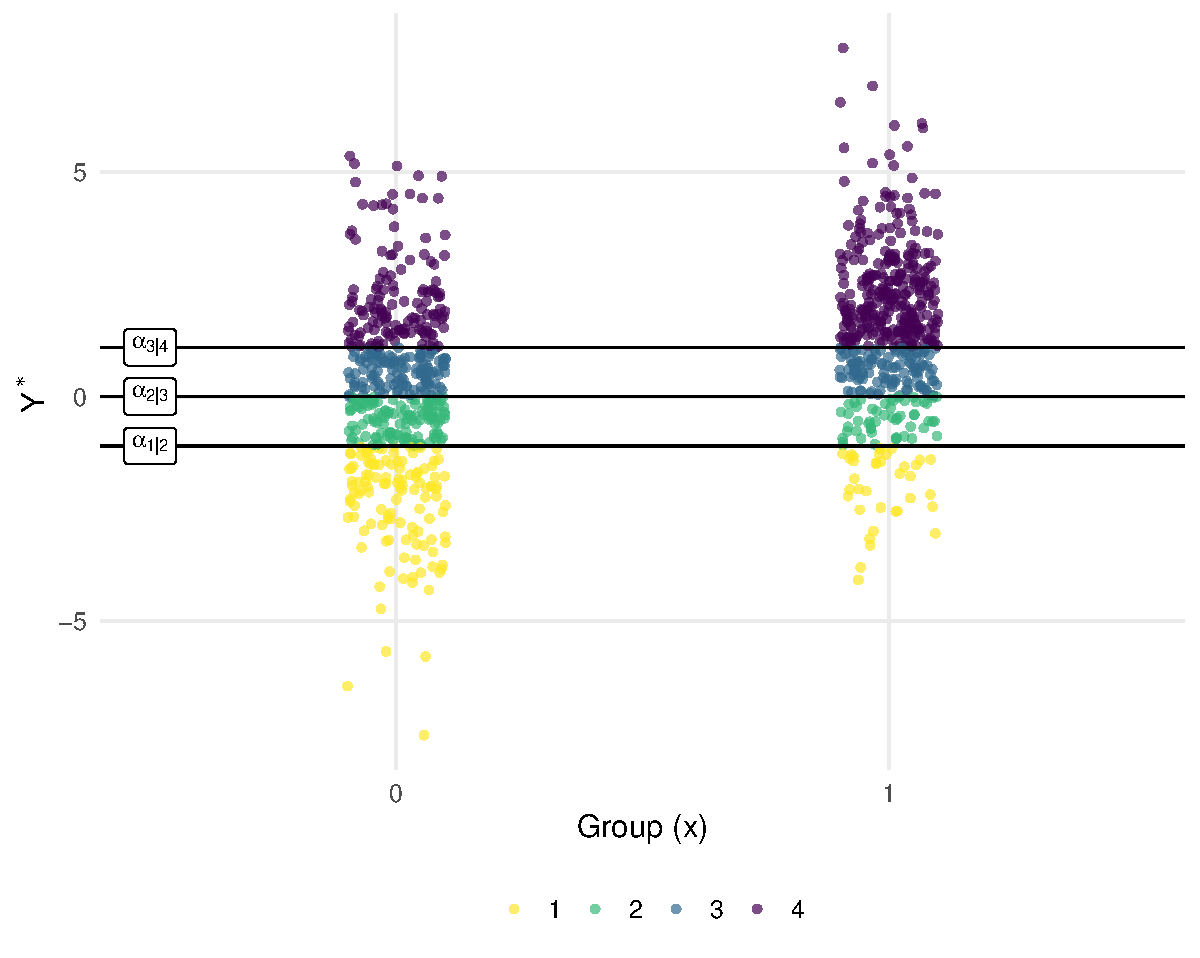
\includegraphics[width=1\linewidth]{paper_files/figure-latex/fig-sim-from-latent-1} 

}

\caption{Example of cutting a latent variable for \(k = 4\) ordinal outcomes with the effect of a binary predictor \(x\). The thresholds are fixed and the difference between the latent means of the two groups increase the number of points (thus probability) in higher outcomes.}\label{fig:fig-sim-from-latent}
\end{figure}

\begin{center}\textbf{[Figure 5 about here]} \end{center}

\normalsize

\scriptsize

\begin{Shaded}
\begin{Highlighting}[]
\NormalTok{dat}\SpecialCharTok{$}\NormalTok{y }\OtherTok{\textless{}{-}} \FunctionTok{ordered}\NormalTok{(dat}\SpecialCharTok{$}\NormalTok{y) }\CommentTok{\# make an ordered factor in R where 1 \textless{} 2 \textless{} 3 \textless{} 4}
\NormalTok{fit }\OtherTok{\textless{}{-}} \FunctionTok{clm}\NormalTok{(y }\SpecialCharTok{\textasciitilde{}}\NormalTok{ x, }\AttributeTok{data =}\NormalTok{ dat, }\AttributeTok{link =} \StringTok{"logit"}\NormalTok{)}
\FunctionTok{summary}\NormalTok{(fit)}
\CommentTok{\#\textgreater{} formula: y \textasciitilde{} x}
\CommentTok{\#\textgreater{} data:    dat}
\CommentTok{\#\textgreater{} }
\CommentTok{\#\textgreater{}  link  threshold nobs logLik   AIC     niter max.grad cond.H }
\CommentTok{\#\textgreater{}  logit flexible  1000 {-}1226.66 2461.32 4(0)  2.25e{-}07 1.7e+01}
\CommentTok{\#\textgreater{} }
\CommentTok{\#\textgreater{} Coefficients:}
\CommentTok{\#\textgreater{}   Estimate Std. Error z value Pr(\textgreater{}|z|)    }
\CommentTok{\#\textgreater{} x   1.4078     0.1233   11.41   \textless{}2e{-}16 ***}
\CommentTok{\#\textgreater{} {-}{-}{-}}
\CommentTok{\#\textgreater{} Signif. codes:  0 \textquotesingle{}***\textquotesingle{} 0.001 \textquotesingle{}**\textquotesingle{} 0.01 \textquotesingle{}*\textquotesingle{} 0.05 \textquotesingle{}.\textquotesingle{} 0.1 \textquotesingle{} \textquotesingle{} 1}
\CommentTok{\#\textgreater{} }
\CommentTok{\#\textgreater{} Threshold coefficients:}
\CommentTok{\#\textgreater{}     Estimate Std. Error z value}
\CommentTok{\#\textgreater{} 1|2 {-}1.13646    0.09757 {-}11.648}
\CommentTok{\#\textgreater{} 2|3 {-}0.07934    0.08603  {-}0.922}
\CommentTok{\#\textgreater{} 3|4  0.98793    0.09269  10.658}
\end{Highlighting}
\end{Shaded}

\normalsize

The simulation using the latent formulation of the model is implemented in the \texttt{sim\_ord\_latent()} function. Basically, we define the dataset \texttt{dat} with predictors. Then the model formula is specified within the function as \texttt{location\ =\ \textasciitilde{}} along with the vector of regression coefficients (\texttt{beta}), baseline probabilities (\texttt{prob0}) and the link function. The function return a dataset with the simulated \(Y\) and the latent variable (this is possible only because we simulate the data, otherwise \(Y^{\star}\) cannot be observed by definition).

\scriptsize

\begin{Shaded}
\begin{Highlighting}[]
\FunctionTok{set.seed}\NormalTok{(}\DecValTok{2024}\NormalTok{)}
\NormalTok{N }\OtherTok{\textless{}{-}} \DecValTok{100} \CommentTok{\# sample size}
\NormalTok{or }\OtherTok{\textless{}{-}} \DecValTok{4} \CommentTok{\# odds ratio, higher here just for a more clear plot}
\NormalTok{k }\OtherTok{\textless{}{-}} \DecValTok{4} \CommentTok{\# number of ordinal alternatives}
\NormalTok{probs0 }\OtherTok{\textless{}{-}} \FunctionTok{rep}\NormalTok{(}\DecValTok{1}\SpecialCharTok{/}\NormalTok{k, k) }\CommentTok{\# probabilities for the first group}
\NormalTok{alpha }\OtherTok{\textless{}{-}} \FunctionTok{prob\_to\_alpha}\NormalTok{(probs0, }\AttributeTok{link =} \StringTok{"logit"}\NormalTok{)}
\NormalTok{dat }\OtherTok{\textless{}{-}} \FunctionTok{data.frame}\NormalTok{(}\AttributeTok{x =} \FunctionTok{rep}\NormalTok{(}\FunctionTok{c}\NormalTok{(}\DecValTok{0}\NormalTok{, }\DecValTok{1}\NormalTok{), }\AttributeTok{each =}\NormalTok{ N}\SpecialCharTok{/}\DecValTok{2}\NormalTok{))}

\CommentTok{\# same as the previous simulation}
\NormalTok{dat }\OtherTok{\textless{}{-}} \FunctionTok{sim\_ord\_latent}\NormalTok{(}\AttributeTok{location =} \SpecialCharTok{\textasciitilde{}}\NormalTok{x, }\AttributeTok{beta =} \FunctionTok{log}\NormalTok{(or), }\AttributeTok{prob0 =}\NormalTok{ probs0, }\AttributeTok{data =}\NormalTok{ dat, }\AttributeTok{link =} \StringTok{"logit"}\NormalTok{)}

\FunctionTok{head\_tail}\NormalTok{(dat, }\AttributeTok{n =} \DecValTok{3}\NormalTok{)}
\CommentTok{\#\textgreater{}     x y         ys}
\CommentTok{\#\textgreater{} 1   0 4  1.6356528}
\CommentTok{\#\textgreater{} 2   0 2 {-}0.7497878}
\CommentTok{\#\textgreater{} 3   0 3  0.7554420}
\CommentTok{\#\textgreater{} 98  1 4  1.4134548}
\CommentTok{\#\textgreater{} 99  1 4  5.0032143}
\CommentTok{\#\textgreater{} 100 1 4  1.6703959}
\end{Highlighting}
\end{Shaded}

\normalsize

\subsubsection{Choosing parameters values}\label{choosing-parameters-values}

\paragraph{\texorpdfstring{Thresholds \(\alpha\)}{Thresholds \textbackslash alpha}}\label{thresholds-alpha}

The previous simulation can be easily extended by adding more predictors and their interactions. The crucial part is setting appropriate and empirically meaningful parameters. In the PO model thresholds are usually not of main interest as intercepts in standard linear regression. Thresholds are essentially quantiles of the latent distribution that produced certain \(k\) probabilities. To set meaningful \(\alpha\) values we can convert probabilities into thresholds (\texttt{alpha\_to\_prob()}). The function \texttt{show\_alpha()} produce a meaningful visual representation of using a specific set of thresholds (see Figure \ref{fig:fig-show-th-example}). Thus with two groups for example, the thresholds are the \(k\) probabilities of the ordinal variable \(Y\) for the reference group (when \(x = 0\)).

\scriptsize

\begin{figure}

{\centering 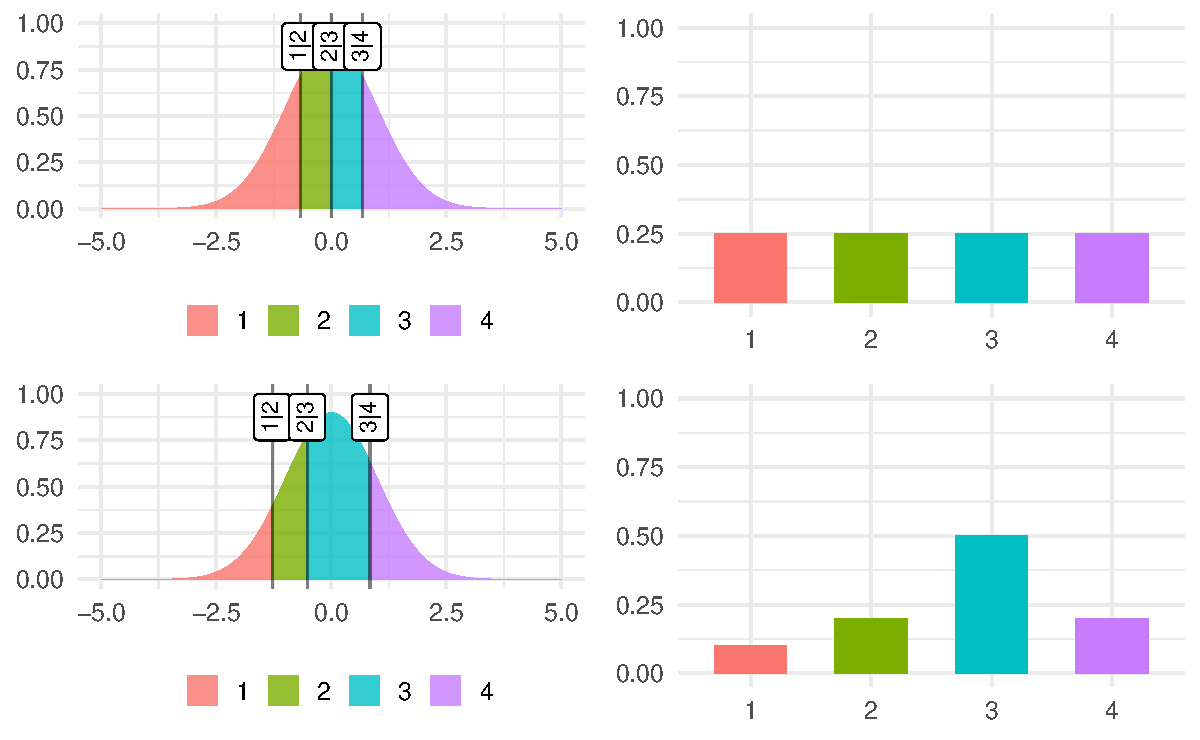
\includegraphics[width=1\linewidth]{paper_files/figure-latex/fig-show-th-example-1} 

}

\caption{Example of the \texttt{show\_alpha()} function. On the left the assumed latent variable and \(k - 1\) thresholds with the corresponding probabilities on the right.}\label{fig:fig-show-th-example}
\end{figure}

\begin{center}\textbf{[Figure 6 about here]} \end{center}

\normalsize

\paragraph{Regression coefficients}\label{regression-coefficients}

For \emph{probit} models we can set the \(\beta_j\) to be in standardized (i.e., Cohen's \(d\)-like) units. For a categorical variable as the previous example with the group, \(\beta_j\) is the degree of separation in standard deviation unit between the two latent distributions. For \emph{logit} models we can set the odds ratio. Meaningful odds ratios can be derived from previous literature, meta-analyses or converting to other effect sizes. For example, Sánchez-Meca, Marín-Martínez, and Chacón-Moscoso (2003) proposed some equations to convert between odds ratios and Cohen's \(d\). Using their approach, a Cohen's \(d = 0.5\) usually considered a plausible medium effect size corresponds to and odds ratio of \(\approx 2.47\).

We can also calculate and plot the predicted probabilities (i.e., \(g^{-1}(\eta)\)) given the predictors and the chosen regression coefficients. In this way we can try different values and see if predicted probabilities are plausible or not. The \texttt{cat\_latent\_plot()} and \texttt{num\_latent\_plot()} functions can be for respectively a categorical (Figures \ref{fig:fig-example-cat-latent}) and numerical predictor (Figures \ref{fig:fig-example-num-latent}). In the supplementary materials we show how to use the \texttt{sim\_ord\_latent()} function for checking the impact of certain \(\beta\) for more complex models.

\scriptsize

\begin{figure}

{\centering 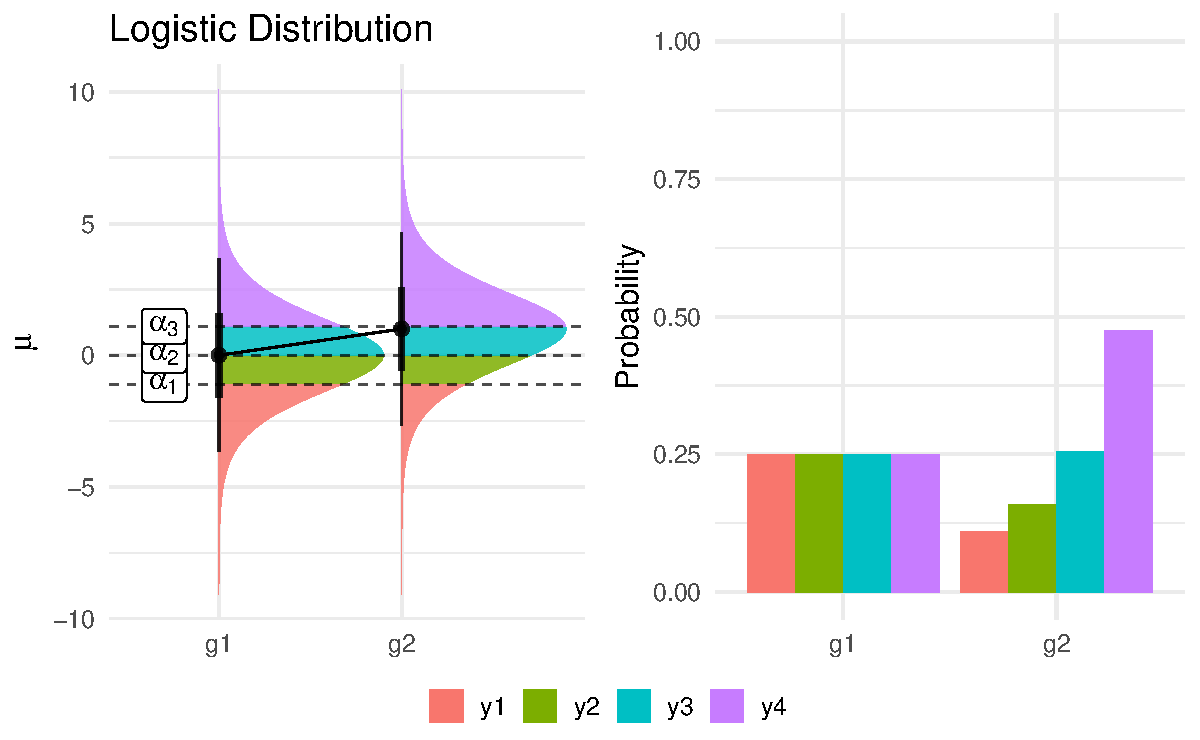
\includegraphics[width=1\linewidth]{paper_files/figure-latex/fig-example-cat-latent-1} 

}

\caption{Example of the \texttt{cat\_latent\_plot()} function depicting the effect of a categorical predictor. On the left the shift in the latent mean and on the right the impact on the expected probabilities. The plot can be created using \texttt{cat\_latent\_plot(m\ =\ c(0,\ 1),\ s\ =\ 1,\ prob0\ =\ rep(1/4,\ 4),\ link\ =\ "logit")}.}\label{fig:fig-example-cat-latent}
\end{figure}

\begin{center}\textbf{[Figure 7 about here]} \end{center}

\normalsize

\scriptsize

\begin{figure}

{\centering 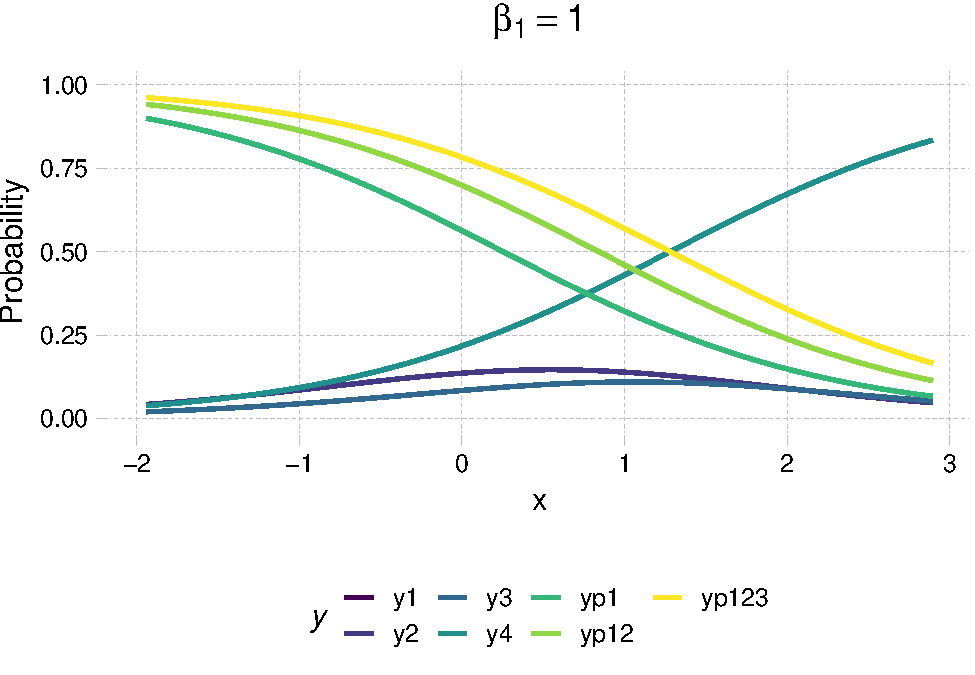
\includegraphics[width=1\linewidth]{paper_files/figure-latex/fig-example-num-latent-1} 

}

\caption{Example of the \texttt{num\_latent\_plot()} function depicting the effect of a continuous predictor on the expected probabilities. Dotted lines are the 25\%, 50\% and 75\% quantiles. \(\beta_1 = 1\) is the regression coefficient. The plot can be created using \texttt{num\_latent\_plot(x\ =\ runif(100),\ b1\ =\ 1,\ prob0\ =\ c(0.6,\ 0.2,\ 0.1,\ 0.1),\ link\ =\ "probit")}}\label{fig:fig-example-num-latent}
\end{figure}

\begin{center}\textbf{[Figure 8 about here]} \end{center}

\normalsize

\subsection{2x2 interaction}\label{x2-interaction}

A common research design could be a 2x2 factorial design. In this example we have two main effects and the interaction. By default R use dummy coding but setting sum-to-zero contrasts (e.g., \(0.5\) and \(-0.5\)) for a factorial design is convenient. In this way \(\beta_1\) will be the main effect of \(X_1\), \(\beta_2\) the main effect of \(X_2\) and \(\beta_3\) the interaction (thus the difference of differences). Equation \eqref{eq:interaction-equation} depict the model formula.

\begin{equation}
P(Y_i \leq k) = g^{-1}[\alpha_k - (\beta_1X_{1_i} + \beta_2X_{2_i} + \beta_3X_{1_i}X_{2_i})]
\label{eq:interaction-equation}
\end{equation}

\scriptsize

\begin{Shaded}
\begin{Highlighting}[]
\FunctionTok{set.seed}\NormalTok{(}\DecValTok{2024}\NormalTok{)}
\NormalTok{n }\OtherTok{\textless{}{-}} \DecValTok{100}
\NormalTok{k }\OtherTok{\textless{}{-}} \DecValTok{3}
\NormalTok{betas }\OtherTok{\textless{}{-}} \FunctionTok{c}\NormalTok{(}\AttributeTok{b1 =} \DecValTok{0}\NormalTok{, }\AttributeTok{b2 =} \DecValTok{1}\NormalTok{, }\AttributeTok{b3 =} \FloatTok{0.5}\NormalTok{) }\CommentTok{\# b1 = main effect X1, b2 = main effect X2, b3 = interaction}

\NormalTok{dat }\OtherTok{\textless{}{-}} \FunctionTok{expand.grid}\NormalTok{(}\AttributeTok{x1 =} \FunctionTok{c}\NormalTok{(}\StringTok{"a"}\NormalTok{, }\StringTok{"b"}\NormalTok{), }\AttributeTok{x2 =} \FunctionTok{c}\NormalTok{(}\StringTok{"c"}\NormalTok{, }\StringTok{"d"}\NormalTok{), }\AttributeTok{n =} \DecValTok{1}\SpecialCharTok{:}\NormalTok{n)}
\NormalTok{dat}\SpecialCharTok{$}\NormalTok{x1 }\OtherTok{\textless{}{-}} \FunctionTok{factor}\NormalTok{(dat}\SpecialCharTok{$}\NormalTok{x1)}
\NormalTok{dat}\SpecialCharTok{$}\NormalTok{x2 }\OtherTok{\textless{}{-}} \FunctionTok{factor}\NormalTok{(dat}\SpecialCharTok{$}\NormalTok{x2)}

\CommentTok{\# sum to 0 coding}
\FunctionTok{contrasts}\NormalTok{(dat}\SpecialCharTok{$}\NormalTok{x1) }\OtherTok{\textless{}{-}} \FunctionTok{c}\NormalTok{(}\FloatTok{0.5}\NormalTok{, }\SpecialCharTok{{-}}\FloatTok{0.5}\NormalTok{)}
\FunctionTok{contrasts}\NormalTok{(dat}\SpecialCharTok{$}\NormalTok{x2) }\OtherTok{\textless{}{-}} \FunctionTok{c}\NormalTok{(}\FloatTok{0.5}\NormalTok{, }\SpecialCharTok{{-}}\FloatTok{0.5}\NormalTok{)}
\NormalTok{probs0 }\OtherTok{\textless{}{-}} \FunctionTok{rep}\NormalTok{(}\DecValTok{1}\SpecialCharTok{/}\NormalTok{k, k)}

\NormalTok{dat }\OtherTok{\textless{}{-}} \FunctionTok{sim\_ord\_latent}\NormalTok{(}\SpecialCharTok{\textasciitilde{}}\NormalTok{ x1 }\SpecialCharTok{*}\NormalTok{ x2, }\AttributeTok{beta =}\NormalTok{ betas, }\AttributeTok{prob0 =}\NormalTok{ probs0, }\AttributeTok{link =} \StringTok{"probit"}\NormalTok{, }\AttributeTok{data =}\NormalTok{ dat)}
\NormalTok{fit }\OtherTok{\textless{}{-}} \FunctionTok{clm}\NormalTok{(y }\SpecialCharTok{\textasciitilde{}}\NormalTok{ x1 }\SpecialCharTok{*}\NormalTok{ x2, }\AttributeTok{data =}\NormalTok{ dat, }\AttributeTok{link =} \StringTok{"probit"}\NormalTok{)}
\FunctionTok{summary}\NormalTok{(fit)}
\CommentTok{\#\textgreater{} formula: y \textasciitilde{} x1 * x2}
\CommentTok{\#\textgreater{} data:    dat}
\CommentTok{\#\textgreater{} }
\CommentTok{\#\textgreater{}  link   threshold nobs logLik  AIC    niter max.grad cond.H }
\CommentTok{\#\textgreater{}  probit flexible  400  {-}390.29 790.57 4(0)  2.20e{-}07 2.1e+01}
\CommentTok{\#\textgreater{} }
\CommentTok{\#\textgreater{} Coefficients:}
\CommentTok{\#\textgreater{}         Estimate Std. Error z value Pr(\textgreater{}|z|)    }
\CommentTok{\#\textgreater{} x11     {-}0.02969    0.11625  {-}0.255    0.798    }
\CommentTok{\#\textgreater{} x21      1.15703    0.11935   9.695   \textless{}2e{-}16 ***}
\CommentTok{\#\textgreater{} x11:x21  0.29058    0.23254   1.250    0.211    }
\CommentTok{\#\textgreater{} {-}{-}{-}}
\CommentTok{\#\textgreater{} Signif. codes:  0 \textquotesingle{}***\textquotesingle{} 0.001 \textquotesingle{}**\textquotesingle{} 0.01 \textquotesingle{}*\textquotesingle{} 0.05 \textquotesingle{}.\textquotesingle{} 0.1 \textquotesingle{} \textquotesingle{} 1}
\CommentTok{\#\textgreater{} }
\CommentTok{\#\textgreater{} Threshold coefficients:}
\CommentTok{\#\textgreater{}     Estimate Std. Error z value}
\CommentTok{\#\textgreater{} 1|2 {-}0.50503    0.06932  {-}7.286}
\CommentTok{\#\textgreater{} 2|3  0.46102    0.06900   6.681}
\end{Highlighting}
\end{Shaded}

\normalsize

The parameters interpretation is the same as introduced in the general case. The thresholds \(\alpha\) are fixed representing the probabilities \(P(Y = k)\) when all predictors are zero. In this case by doing \texttt{alpha\_to\_prob(fit\$alpha,\ link\ =\ "probit")} we should recover the \texttt{probs0} vector. \texttt{x1} is the main effect thus the difference in \(z\) scores between \emph{a} and \emph{b} averaging over \texttt{x2}. The same holds for \texttt{x2}. \texttt{x1:x2} is the interaction thus difference of differences in \(z\) scores (see Figure \ref{fig:fig-effects-2-by-2-interaction}).

\scriptsize

\begin{figure}

{\centering 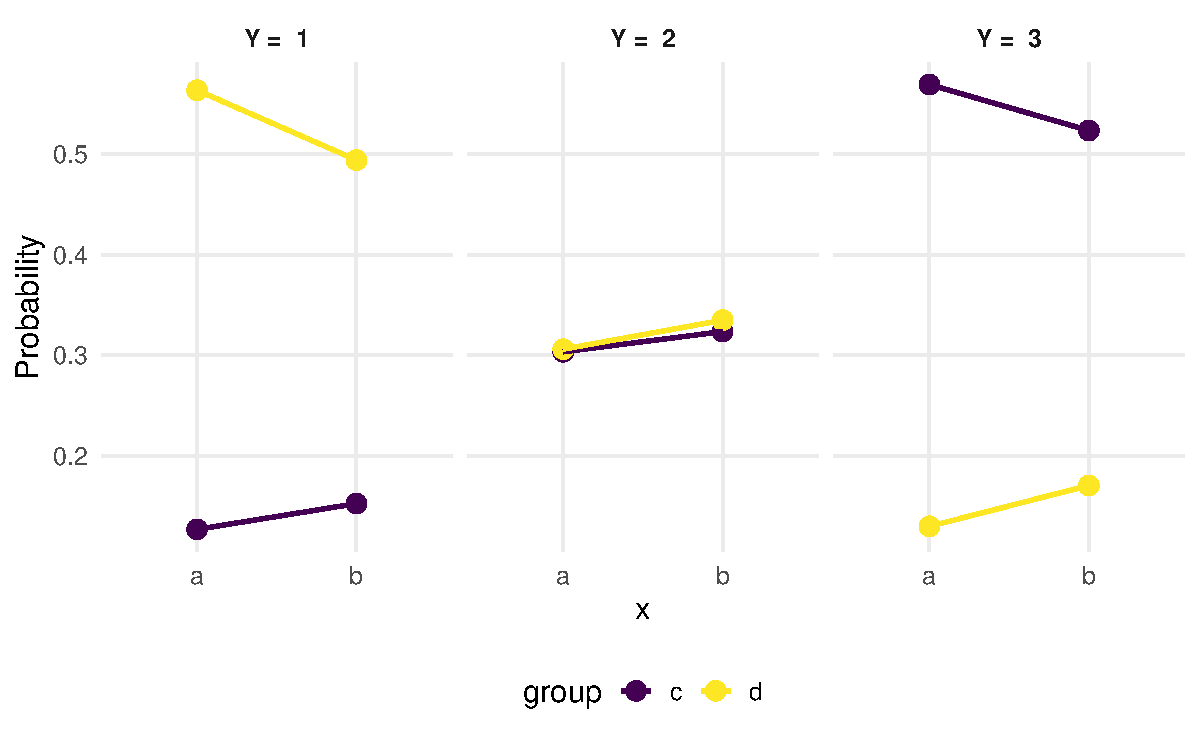
\includegraphics[width=1\linewidth]{paper_files/figure-latex/fig-effects-2-by-2-interaction-1} 

}

\caption{Results from the simulated model with a 2x2 interaction between categorical predictors. The plot shows the predicted probabilities for each ordinal outcome as a function of the two predictors. A similar plot can be produced using \texttt{plot(ggeffects::ggpredict(fit,\ terms\ =\ c("x1",\ "x2")))}.}\label{fig:fig-effects-2-by-2-interaction}
\end{figure}

\begin{center}\textbf{[Figure 9 about here]} \end{center}

\normalsize

\subsection{Numerical by categorical interaction}\label{numerical-by-categorical-interaction}

Another common scenario is the interaction between a numerical variable \(x\) and a categorical variable \(g\). For simplicity we simulate the factor with two levels and the numerical variable sampled from an uniform distribution between 0 and 1.

\scriptsize

\begin{Shaded}
\begin{Highlighting}[]
\FunctionTok{set.seed}\NormalTok{(}\DecValTok{2024}\NormalTok{)}
\NormalTok{n }\OtherTok{\textless{}{-}} \DecValTok{100}
\NormalTok{k }\OtherTok{\textless{}{-}} \DecValTok{3}
\NormalTok{dat }\OtherTok{\textless{}{-}} \FunctionTok{data.frame}\NormalTok{(}\AttributeTok{x =} \FunctionTok{runif}\NormalTok{(n),}
                  \AttributeTok{g =} \FunctionTok{rep}\NormalTok{(}\FunctionTok{c}\NormalTok{(}\StringTok{"a"}\NormalTok{, }\StringTok{"b"}\NormalTok{), }\AttributeTok{each =}\NormalTok{ n}\SpecialCharTok{/}\DecValTok{2}\NormalTok{))}
\NormalTok{dat}\SpecialCharTok{$}\NormalTok{g }\OtherTok{\textless{}{-}} \FunctionTok{factor}\NormalTok{(dat}\SpecialCharTok{$}\NormalTok{g)}
\FunctionTok{contrasts}\NormalTok{(dat}\SpecialCharTok{$}\NormalTok{g) }\OtherTok{\textless{}{-}} \FunctionTok{c}\NormalTok{(}\FloatTok{0.5}\NormalTok{, }\SpecialCharTok{{-}}\FloatTok{0.5}\NormalTok{)}
\NormalTok{probs0 }\OtherTok{\textless{}{-}} \FunctionTok{rep}\NormalTok{(}\DecValTok{1}\SpecialCharTok{/}\NormalTok{k, k)}

\NormalTok{dat }\OtherTok{\textless{}{-}} \FunctionTok{sim\_ord\_latent}\NormalTok{(}\SpecialCharTok{\textasciitilde{}}\NormalTok{ x }\SpecialCharTok{*}\NormalTok{ g, }\AttributeTok{beta =} \FunctionTok{c}\NormalTok{(}\FloatTok{0.3}\NormalTok{, }\FloatTok{0.5}\NormalTok{, }\FloatTok{0.5}\NormalTok{), }\AttributeTok{prob0 =}\NormalTok{ probs0, }\AttributeTok{link =} \StringTok{"probit"}\NormalTok{, }\AttributeTok{data =}\NormalTok{ dat)}
\NormalTok{fit }\OtherTok{\textless{}{-}} \FunctionTok{clm}\NormalTok{(y }\SpecialCharTok{\textasciitilde{}}\NormalTok{ x }\SpecialCharTok{*}\NormalTok{ g, }\AttributeTok{data =}\NormalTok{ dat, }\AttributeTok{link =} \StringTok{"probit"}\NormalTok{)}
\FunctionTok{summary}\NormalTok{(fit)}
\CommentTok{\#\textgreater{} formula: y \textasciitilde{} x * g}
\CommentTok{\#\textgreater{} data:    dat}
\CommentTok{\#\textgreater{} }
\CommentTok{\#\textgreater{}  link   threshold nobs logLik  AIC    niter max.grad cond.H }
\CommentTok{\#\textgreater{}  probit flexible  100  {-}101.63 213.26 5(0)  3.01e{-}08 1.0e+02}
\CommentTok{\#\textgreater{} }
\CommentTok{\#\textgreater{} Coefficients:}
\CommentTok{\#\textgreater{}      Estimate Std. Error z value Pr(\textgreater{}|z|)  }
\CommentTok{\#\textgreater{} x     0.68616    0.40959   1.675   0.0939 .}
\CommentTok{\#\textgreater{} g1    0.07207    0.45768   0.157   0.8749  }
\CommentTok{\#\textgreater{} x:g1  1.21471    0.81881   1.484   0.1379  }
\CommentTok{\#\textgreater{} {-}{-}{-}}
\CommentTok{\#\textgreater{} Signif. codes:  0 \textquotesingle{}***\textquotesingle{} 0.001 \textquotesingle{}**\textquotesingle{} 0.01 \textquotesingle{}*\textquotesingle{} 0.05 \textquotesingle{}.\textquotesingle{} 0.1 \textquotesingle{} \textquotesingle{} 1}
\CommentTok{\#\textgreater{} }
\CommentTok{\#\textgreater{} Threshold coefficients:}
\CommentTok{\#\textgreater{}     Estimate Std. Error z value}
\CommentTok{\#\textgreater{} 1|2  {-}0.1059     0.2352  {-}0.450}
\CommentTok{\#\textgreater{} 2|3   0.6529     0.2408   2.711}
\end{Highlighting}
\end{Shaded}

\normalsize

Again, \texttt{x} is the slope of the numerical predictor averaging over \texttt{g} (given that \texttt{g} has been coded with sum-to-zero contrasts) thus the increase in \(z\) scores for a unit increase in \texttt{x}. \texttt{g1} is the main effect of the factor evaluated when \(x = 0\) (centering \(x\) will change the parameter interpretation). The \texttt{x:g1} is the slopes difference the two groups. Figure \ref{fig:fig-effects-num-by-cat-interaction} depicts the model results.

\scriptsize

\begin{figure}

{\centering 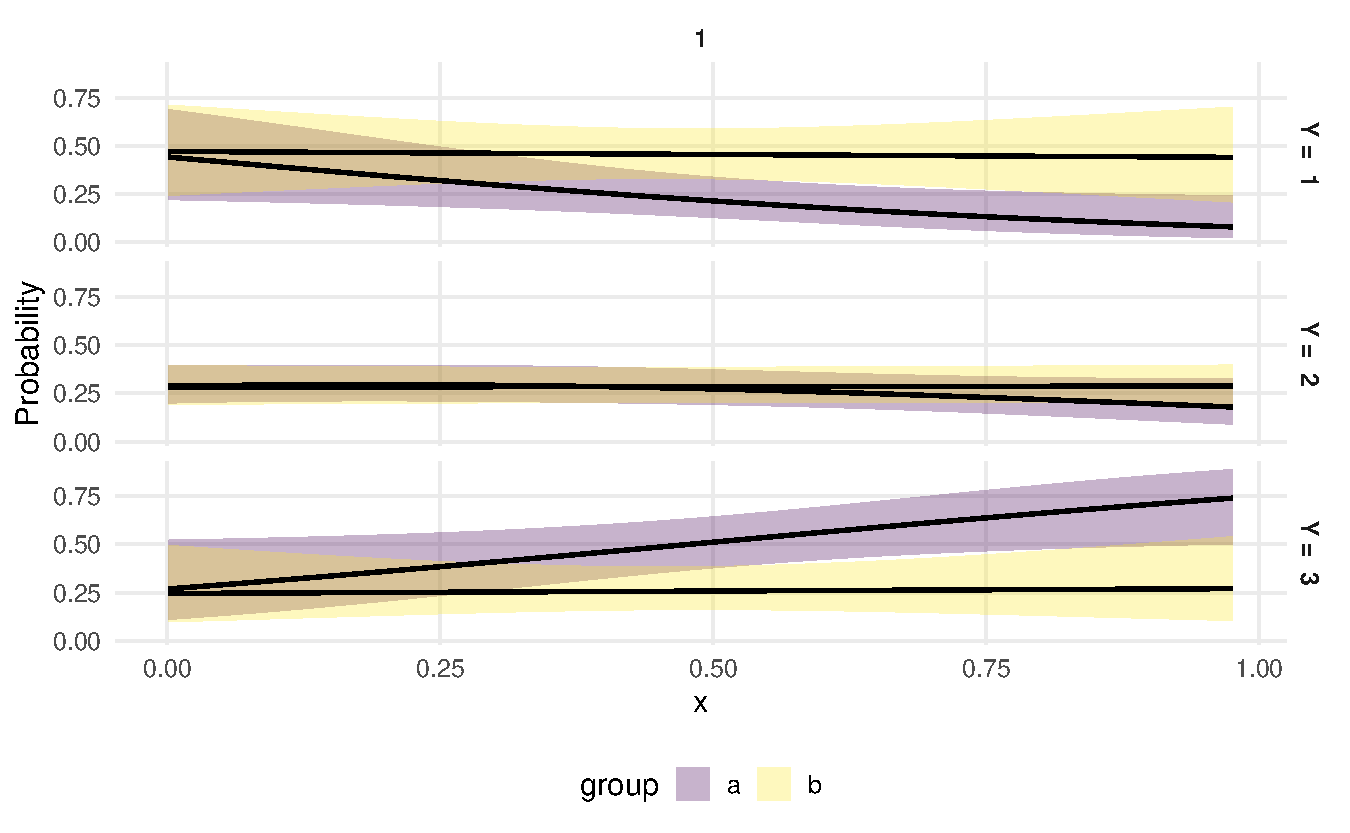
\includegraphics[width=1\linewidth]{paper_files/figure-latex/fig-effects-num-by-cat-interaction-1} 

}

\caption{Results from the simulated model with the interaction between a continuous and categorical variables. The plot shows the predicted probabilities with 95\% confidence intervals as a function of predictors. A similar plot can be produced using \texttt{plot(ggeffects::ggpredict(fit,\ terms\ =\ c("x{[}all{]}",\ "g")))}}\label{fig:fig-effects-num-by-cat-interaction}
\end{figure}

\begin{center}\textbf{[Figure 10 about here]} \end{center}

\normalsize

\section{Power Analysis}\label{power-analysis}

In this section we introduce how to estimate the statistical power. Power analysis is a crucial and often necessary step when planning a confirmatory study (Lakens, 2022) or preparing a pre-registration or registered report (Chambers \& Tzavella, 2022). Furthermore, statistical power for complex models can only be estimated using Monte Carlo simulations.

Formally the power is defined as the probability of correctly rejecting the null hypothesis \(H_0\). For simple cases (e.g., a t-test) the power can be calculated analytically while in complex cases simulating data is the best approach. We present very general example that, as for the previous simulations, can be easily extended.

The general workflow for a power simulation can be summarized as:

\begin{enumerate}
\def\labelenumi{\arabic{enumi}.}
\tightlist
\item
  Specify the research design, e.g., 2x2 factorial design
\item
  Specify the effect/parameter of interest, e.g., the interaction effect
\item
  Define the simulation conditions, e.g., a range of sample size, effect size, etc.
\item
  Implement one of the simulation workflow described in the previous sections
\item
  Repeat the simulation a large number of times (e.g, 10000) and store the relevant values from each simulation
\item
  Summarise the simulation results
\end{enumerate}

We can estimate the power of detecting a group difference of \(d = 0.4\) (assuming a \emph{probit} model). Participants respond to an ordinal variable with \(k = 5\). The simulation is performed using a \texttt{for} loop that repeat 1000 times the data simulation, model fitting and extract the p-value for the \(\beta_1\). The power is then estimated as the number of p-values lower than the critical level over the number of simulations.

\scriptsize

\begin{Shaded}
\begin{Highlighting}[]
\FunctionTok{set.seed}\NormalTok{(}\DecValTok{2024}\NormalTok{)}
\NormalTok{n }\OtherTok{\textless{}{-}} \DecValTok{40} \CommentTok{\# sample size}
\NormalTok{k }\OtherTok{\textless{}{-}} \DecValTok{5}  \CommentTok{\# number of ordinal variables}
\NormalTok{d }\OtherTok{\textless{}{-}} \FloatTok{0.4} \CommentTok{\# effect size (i.e., our regression coefficients)}
\NormalTok{nsim }\OtherTok{\textless{}{-}} \FloatTok{1e3} \CommentTok{\# higher is better, here using 1000 for an example}
\NormalTok{probs0 }\OtherTok{\textless{}{-}} \FunctionTok{rep}\NormalTok{(}\DecValTok{1}\SpecialCharTok{/}\NormalTok{k, k)}
\NormalTok{alpha }\OtherTok{\textless{}{-}} \FloatTok{0.05} \CommentTok{\# critical alpha}

\NormalTok{p }\OtherTok{\textless{}{-}} \FunctionTok{rep}\NormalTok{(}\ConstantTok{NA}\NormalTok{, nsim) }\CommentTok{\# preallocation to improve loop computational efficiency}
\NormalTok{dat }\OtherTok{\textless{}{-}} \FunctionTok{data.frame}\NormalTok{(}\AttributeTok{group =} \FunctionTok{rep}\NormalTok{(}\FunctionTok{c}\NormalTok{(}\StringTok{"a"}\NormalTok{, }\StringTok{"b"}\NormalTok{), }\AttributeTok{each =}\NormalTok{ n)) }\CommentTok{\# data frame}

\FunctionTok{head\_tail}\NormalTok{(dat, }\AttributeTok{n =} \DecValTok{3}\NormalTok{)}
\CommentTok{\#\textgreater{}    group}
\CommentTok{\#\textgreater{} 1      a}
\CommentTok{\#\textgreater{} 2      a}
\CommentTok{\#\textgreater{} 3      a}
\CommentTok{\#\textgreater{} 78     b}
\CommentTok{\#\textgreater{} 79     b}
\CommentTok{\#\textgreater{} 80     b}

\ControlFlowTok{for}\NormalTok{(i }\ControlFlowTok{in} \DecValTok{1}\SpecialCharTok{:}\NormalTok{nsim)\{}
\NormalTok{  sim }\OtherTok{\textless{}{-}} \FunctionTok{sim\_ord\_latent}\NormalTok{(}\SpecialCharTok{\textasciitilde{}}\NormalTok{group, }\AttributeTok{beta =}\NormalTok{ d, }\AttributeTok{prob0 =}\NormalTok{ probs0, }\AttributeTok{link =} \StringTok{"probit"}\NormalTok{, }\AttributeTok{data =}\NormalTok{ dat)}
\NormalTok{  fit }\OtherTok{\textless{}{-}} \FunctionTok{clm}\NormalTok{(y }\SpecialCharTok{\textasciitilde{}}\NormalTok{ group, }\AttributeTok{data =}\NormalTok{ sim, }\AttributeTok{link =} \StringTok{"probit"}\NormalTok{)}
\NormalTok{  p[i] }\OtherTok{\textless{}{-}} \FunctionTok{summary}\NormalTok{(fit)}\SpecialCharTok{$}\NormalTok{coefficients[}\StringTok{"groupb"}\NormalTok{, }\StringTok{"Pr(\textgreater{}|z|)"}\NormalTok{] }\CommentTok{\# extract the pvalue}
\NormalTok{\}}

\CommentTok{\# estimate the power}
\FunctionTok{mean}\NormalTok{(p }\SpecialCharTok{\textless{}=}\NormalTok{ alpha, }\AttributeTok{na.rm =} \ConstantTok{TRUE}\NormalTok{)}
\CommentTok{\#\textgreater{} [1] 0.418}
\end{Highlighting}
\end{Shaded}

\normalsize

Despite useful, calculating power curves instead a single value is more informative. For this reason we repeat the previous simulation but for different sample sizes. Figure \ref{fig:fig-power-curve} depict the power curve resulting from the simulation.

\scriptsize

\begin{Shaded}
\begin{Highlighting}[]
\FunctionTok{set.seed}\NormalTok{(}\DecValTok{2024}\NormalTok{)}

\NormalTok{n }\OtherTok{\textless{}{-}} \FunctionTok{c}\NormalTok{(}\DecValTok{20}\NormalTok{, }\DecValTok{40}\NormalTok{, }\DecValTok{60}\NormalTok{, }\DecValTok{100}\NormalTok{, }\DecValTok{200}\NormalTok{)}
\NormalTok{power }\OtherTok{\textless{}{-}} \FunctionTok{rep}\NormalTok{(}\ConstantTok{NA}\NormalTok{, }\FunctionTok{length}\NormalTok{(n))}

\ControlFlowTok{for}\NormalTok{(i }\ControlFlowTok{in} \DecValTok{1}\SpecialCharTok{:}\FunctionTok{length}\NormalTok{(n))\{}
\NormalTok{  p }\OtherTok{\textless{}{-}} \FunctionTok{rep}\NormalTok{(}\ConstantTok{NA}\NormalTok{, nsim) }\CommentTok{\# preallocation for speed}
\NormalTok{  dat }\OtherTok{\textless{}{-}} \FunctionTok{data.frame}\NormalTok{(}\AttributeTok{group =} \FunctionTok{rep}\NormalTok{(}\FunctionTok{c}\NormalTok{(}\StringTok{"a"}\NormalTok{, }\StringTok{"b"}\NormalTok{), }\AttributeTok{each =}\NormalTok{ n[i]))}
  \ControlFlowTok{for}\NormalTok{(j }\ControlFlowTok{in} \DecValTok{1}\SpecialCharTok{:}\NormalTok{nsim)\{}
\NormalTok{    sim }\OtherTok{\textless{}{-}} \FunctionTok{sim\_ord\_latent}\NormalTok{(}\SpecialCharTok{\textasciitilde{}}\NormalTok{group, }\AttributeTok{beta =}\NormalTok{ d, }\AttributeTok{prob0 =}\NormalTok{ probs0, }\AttributeTok{link =} \StringTok{"probit"}\NormalTok{, }\AttributeTok{data =}\NormalTok{ dat)}
\NormalTok{    fit }\OtherTok{\textless{}{-}} \FunctionTok{clm}\NormalTok{(y }\SpecialCharTok{\textasciitilde{}}\NormalTok{ group, }\AttributeTok{data =}\NormalTok{ sim, }\AttributeTok{link =} \StringTok{"probit"}\NormalTok{)}
\NormalTok{    p[j] }\OtherTok{\textless{}{-}} \FunctionTok{summary}\NormalTok{(fit)}\SpecialCharTok{$}\NormalTok{coefficients[}\StringTok{"groupb"}\NormalTok{, }\StringTok{"Pr(\textgreater{}|z|)"}\NormalTok{]}
\NormalTok{  \}}
\NormalTok{  power[i] }\OtherTok{\textless{}{-}} \FunctionTok{mean}\NormalTok{(p }\SpecialCharTok{\textless{}=}\NormalTok{ alpha)}
\NormalTok{\}}

\NormalTok{power}
\CommentTok{\#\textgreater{} [1] 0.225 0.412 0.522 0.750 0.964}
\end{Highlighting}
\end{Shaded}

\normalsize

\scriptsize

\begin{figure}

{\centering 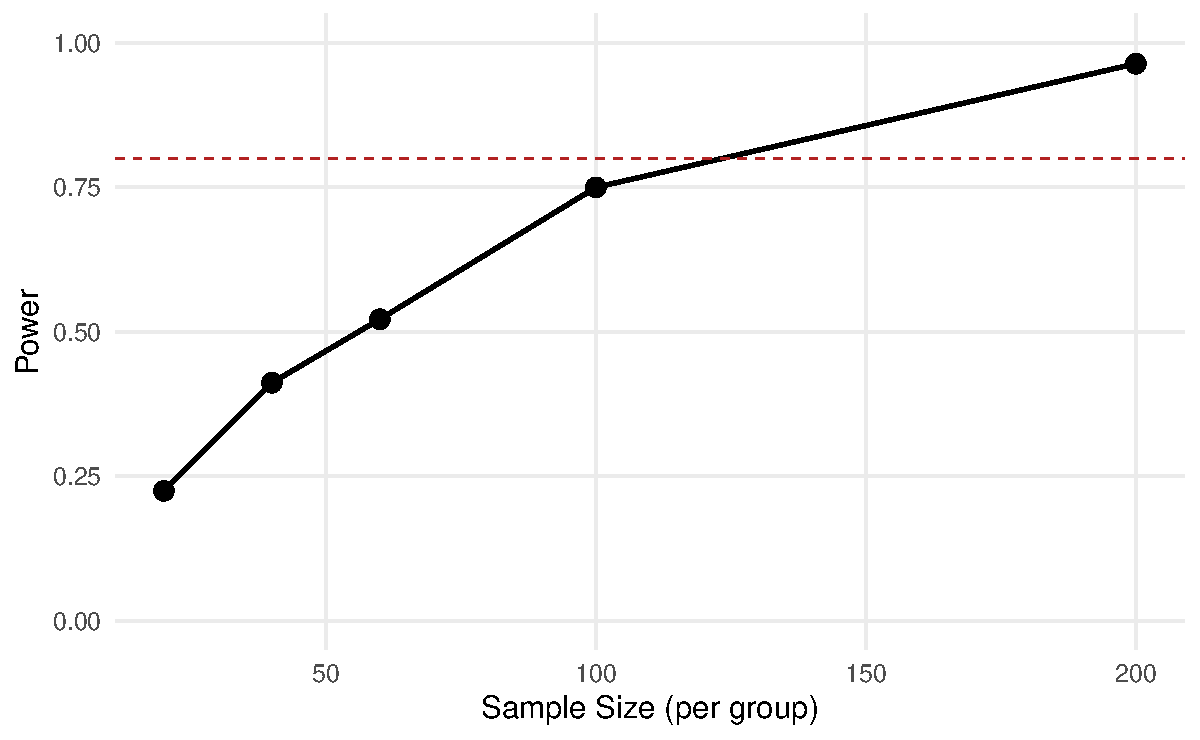
\includegraphics[width=1\linewidth]{paper_files/figure-latex/fig-power-curve-1} 

}

\caption{Results from the power analysis. The x-axis represents the sample size (per group) and the y axis the estimated power. The red dotted line highlight the 80\% power level.}\label{fig:fig-power-curve}
\end{figure}

\begin{center}\textbf{[Figure 11 about here]} \end{center}

\normalsize

\newpage

\section{References}\label{references}

\phantomsection\label{refs}
\begin{CSLReferences}{1}{0}
\bibitem[\citeproctext]{ref-Agresti2010-rz}
Agresti, A. (2010). \emph{Analysis of ordinal categorical data}. Hoboken, NJ, USA: John Wiley \& Sons, Inc. \url{https://doi.org/10.1002/9780470594001}

\bibitem[\citeproctext]{ref-Burkner2019-aw}
Bürkner, P.-C., \& Vuorre, M. (2019). Ordinal regression models in psychology: A tutorial. \emph{Advances in Methods and Practices in Psychological Science}, \emph{2}, 77--101. \url{https://doi.org/10.1177/2515245918823199}

\bibitem[\citeproctext]{ref-Carifio2008-qd}
Carifio, J., \& Perla, R. (2008). Resolving the 50-year debate around using and misusing likert scales. \emph{Medical Education}, \emph{42}, 1150--1152. \url{https://doi.org/10.1111/j.1365-2923.2008.03172.x}

\bibitem[\citeproctext]{ref-Carifio2007-kk}
Carifio, J., \& Perla, R. J. (2007). Ten common misunderstandings, misconceptions, persistent myths and urban legends about likert scales and likert response formats and their antidotes. \emph{Journal of Social Sciences}, \emph{3}, 106--116. \url{https://doi.org/10.3844/jssp.2007.106.116}

\bibitem[\citeproctext]{ref-Chambers2022-tz}
Chambers, C. D., \& Tzavella, L. (2022). The past, present and future of registered reports. \emph{Nature Human Behaviour}, \emph{6}, 29--42. \url{https://doi.org/10.1038/s41562-021-01193-7}

\bibitem[\citeproctext]{ref-Christensen2019-cz}
Christensen, R. H. B. (2019). \emph{Ordinal---regression models for ordinal data}.

\bibitem[\citeproctext]{ref-Christensen2022-jk}
Christensen, R. H. B. (2022). \emph{Ordinal---regression models for ordinal data}.

\bibitem[\citeproctext]{ref-Cliff1996-qo}
Cliff, N. (1996). Answering ordinal questions with ordinal data using ordinal statistics. \emph{Multivariate Behavioral Research}, \emph{31}, 331--350. \url{https://doi.org/10.1207/s15327906mbr3103_4}

\bibitem[\citeproctext]{ref-Cliff2016-ck}
Cliff, Norman. (2016). \emph{Ordinal methods for behavioral data analysis}. London, England: Psychology Press.

\bibitem[\citeproctext]{ref-Cox1995-ur}
Cox, C. (1995). Location-scale cumulative odds models for ordinal data: A generalized non-linear model approach. \emph{Statistics in Medicine}, \emph{14}, 1191--1203. \url{https://doi.org/10.1002/sim.4780141105}

\bibitem[\citeproctext]{ref-DeBruine2021-id}
DeBruine, L. M., \& Barr, D. J. (2021). Understanding mixed-effects models through data simulation. \emph{Advances in Methods and Practices in Psychological Science}, \emph{4}, 2515245920965119. \url{https://doi.org/10.1177/2515245920965119}

\bibitem[\citeproctext]{ref-DeCarlo2010-lj}
DeCarlo, L. T. (2010). On the statistical and theoretical basis of signal detection theory and extensions: Unequal variance, random coefficient, and mixture models. \emph{Journal of Mathematical Psychology}, \emph{54}, 304--313. \url{https://doi.org/10.1016/j.jmp.2010.01.001}

\bibitem[\citeproctext]{ref-Fox2015-ps}
Fox, J. (2015). \emph{Applied regression analysis and generalized linear models}. SAGE Publications. Retrieved from \url{https://play.google.com/store/books/details?id=BlsKogEACAAJ}

\bibitem[\citeproctext]{ref-Gambarota2023-on}
Gambarota, F., \& Altoè, G. (2023). Understanding meta-analysis through data simulation with applications to power analysis. \emph{Advances in Methods and Practices in Psychological Science}. \url{https://doi.org/10.1177/25152459231209330}

\bibitem[\citeproctext]{ref-Gelman2020-tg}
Gelman, A., Hill, J., \& Vehtari, A. (2020). \emph{Regression and other stories}. Cambridge University Press. \url{https://doi.org/10.1017/9781139161879}

\bibitem[\citeproctext]{ref-Jamieson2004-xf}
Jamieson, S. (2004). Likert scales: How to (ab)use them. \emph{Medical Education}, \emph{38}, 1217--1218. \url{https://doi.org/10.1111/j.1365-2929.2004.02012.x}

\bibitem[\citeproctext]{ref-Kemp2021-dj}
Kemp, S., \& Grace, R. C. (2021). Using ordinal scales in psychology. \emph{Methods in Psychology (Online)}, \emph{5}, 100054. \url{https://doi.org/10.1016/j.metip.2021.100054}

\bibitem[\citeproctext]{ref-Kruschke2015-re}
Kruschke, J. K. (2015). \emph{Doing bayesian data analysis}. \url{https://doi.org/10.1016/c2012-0-00477-2}

\bibitem[\citeproctext]{ref-Lakens2022-jp}
Lakens, D. (2022). Sample size justification. \emph{Collabra. Psychology}, \emph{8}. \url{https://doi.org/10.1525/collabra.33267}

\bibitem[\citeproctext]{ref-Liddell2018-wu}
Liddell, T. M., \& Kruschke, J. K. (2018). Analyzing ordinal data with metric models: What could possibly go wrong? \emph{Journal of Experimental Social Psychology}, \emph{79}, 328--348. \url{https://doi.org/10.1016/j.jesp.2018.08.009}

\bibitem[\citeproctext]{ref-Likert1932-xw}
Likert, R. (1932). A technique for the measurement of attitudes. \emph{Archives of Psychology}, \emph{22}, 55. Retrieved from \url{https://psycnet.apa.org/record/1933-01885-001}

\bibitem[\citeproctext]{ref-Liu2023-bp}
Liu, A., He, H., Tu, X. M., \& Tang, W. (2023). On testing proportional odds assumptions for proportional odds models. \emph{General Psychiatry}, \emph{36}, e101048. \url{https://doi.org/10.1136/gpsych-2023-101048}

\bibitem[\citeproctext]{ref-McCullagh1980-cw}
McCullagh, P. (1980). Regression models for ordinal data. \emph{Journal of the Royal Statistical Society}, \emph{42}, 109--127. \url{https://doi.org/10.1111/j.2517-6161.1980.tb01109.x}

\bibitem[\citeproctext]{ref-Overgaard2021-hs}
Overgaard, M., \& Sandberg, K. (2021). The perceptual awareness scale---recent controversies and debates. \emph{Neuroscience of Consciousness}. Retrieved from \url{https://academic.oup.com/nc/article-pdf/doi/10.1093/nc/niab044/41765024/niab044.pdf}

\bibitem[\citeproctext]{ref-Peterson1990-cz}
Peterson, B., \& Harrell, F. E. (1990). Partial proportional odds models for ordinal response variables. \emph{Journal of the Royal Statistical Society. Series C, Applied Statistics}, \emph{39}, 205. \url{https://doi.org/10.2307/2347760}

\bibitem[\citeproctext]{ref-R-base}
R Core Team. (2023). \emph{R: A language and environment for statistical computing}. Vienna, Austria: R Foundation for Statistical Computing. Retrieved from \url{https://www.R-project.org/}

\bibitem[\citeproctext]{ref-Rigby2005-ko}
Rigby, R. A., \& Stasinopoulos, D. M. (2005). Generalized additive models for location, scale and shape. \emph{Journal of the Royal Statistical Society. Series C, Applied Statistics}, \emph{54}, 507--554. \url{https://doi.org/10.1111/j.1467-9876.2005.00510.x}

\bibitem[\citeproctext]{ref-Robitzsch2020-la}
Robitzsch, A. (2020). Why ordinal variables can (almost) always be treated as continuous variables: Clarifying assumptions of robust continuous and ordinal factor analysis estimation methods. \emph{Frontiers in Education}, \emph{5}, 589965. \url{https://doi.org/10.3389/feduc.2020.589965}

\bibitem[\citeproctext]{ref-Sanchez-Meca2003-ji}
Sánchez-Meca, J., Marín-Martínez, F., \& Chacón-Moscoso, S. (2003). Effect-size indices for dichotomized outcomes in meta-analysis. \emph{Psychological Methods}, \emph{8}, 448--467. \url{https://doi.org/10.1037/1082-989X.8.4.448}

\bibitem[\citeproctext]{ref-Schad2020-ht}
Schad, D. J., Vasishth, S., Hohenstein, S., \& Kliegl, R. (2020). How to capitalize on a priori contrasts in linear (mixed) models: A tutorial. \emph{Journal of Memory and Language}, \emph{110}, 104038. \url{https://doi.org/10.1016/j.jml.2019.104038}

\bibitem[\citeproctext]{ref-Stevens1946-te}
Stevens, S. S. (1946). On the theory of scales of measurement. \emph{Science (New York, N.Y.)}, \emph{103}, 677--680. \url{https://doi.org/10.1126/science.103.2684.677}

\bibitem[\citeproctext]{ref-Tutz1990-fe}
Tutz, G. (1990). Sequential item response models with an ordered response. \emph{The British Journal of Mathematical and Statistical Psychology}, \emph{43}, 39--55. \url{https://doi.org/10.1111/j.2044-8317.1990.tb00925.x}

\bibitem[\citeproctext]{ref-Tutz2022-dg}
Tutz, G. (2022). Ordinal regression: A review and a taxonomy of models. \emph{Wiley Interdisciplinary Reviews. Computational Statistics}, \emph{14}. \url{https://doi.org/10.1002/wics.1545}

\bibitem[\citeproctext]{ref-Tutz2020-xq}
Tutz, G., \& Berger, M. (2020). Non proportional odds models are widely dispensable -- sparser modeling based on parametric and additive location-shift approaches. \emph{arXiv {[}Stat.ME{]}}. Retrieved from \url{http://arxiv.org/abs/2006.03914}

\end{CSLReferences}
































\end{document}
